% Combined capstone report: MNIST and Fashion-MNIST.
% Layout follows the program's sample capstone report (scrartcl, title page with abstract, table of contents).

\documentclass{scrartcl}

% Adapted from an original template by Hlyni Arnórssyni, Reykjavik University, Iceland
%
% ------------------------------ SETTINGS
\usepackage{geometry}

\geometry{
	paper=a4paper, % Paper size
	top=2.5cm, % Top margin
	bottom=2.5cm, % Bottom margin
	left=2.5cm, % Left margin
	right=2.4cm, % Right margin
	headheight=0.75cm, % Header height
	footskip=1.5cm, % Space from the bottom margin to the baseline of the footer
	headsep=0.75cm, % Space from the top margin to the baseline of the header
	%showframe, % Uncomment to show how the type block is set on the page
}

\usepackage{blindtext}
%-------------------------------- Character encoding ----------------------------
\usepackage[T1]{fontenc}
\usepackage[utf8]{inputenc}

%----------------------------- Mathematics packages from AMS ---------------

\usepackage{amsmath, amsfonts, amsthm, amssymb}
\usepackage{braket, nicefrac}

% ----------- International System of Units
\usepackage{siunitx}

%------------------------------ Lists / numbers -------------------------
\usepackage{enumitem, multicol}

%------------------------------- Figure insertions --------------
\usepackage{graphicx, float}  % Use option [H] to force the placement of a figure
\usepackage{keystroke}
\usepackage{pgfplots}\usepgfplotslibrary{units}\pgfplotsset{compat=1.16}




%%%%%%%%%%%%%%%%%%%%%%%%%% Hyperlink References %%%%%%%%%%%%%%%%%%%%%%%%%%%
\usepackage{hyperref}

%--------------------% Storage Path for images %-----------------%
\graphicspath{{graphics/}{Graphics/}{./}}
\usepackage{graphicx}
\usepackage{array, booktabs, tabularx, multirow}
\usepackage{xcolor}
\usepackage{caption}
\captionsetup[figure]{name=Fig., labelsep=period, font=small, justification=justified, singlelinecheck=true}
\captionsetup[table]{name=TABLE, labelsep=newline, font=small, labelfont=normalfont, textfont=sc, justification=centering, skip=4pt}
\renewcommand{\thetable}{\Roman{table}}
\usetikzlibrary{arrows.meta, positioning}
\definecolor{GWBlue}{RGB}{0,51,102}
\newcolumntype{C}[1]{>{\centering\arraybackslash}p{#1}}
\newcolumntype{L}[1]{>{\raggedright\arraybackslash}p{#1}}
\hypersetup{
   colorlinks   = true,
   urlcolor     = blue,
   linkcolor    = blue,
   citecolor    = red,
   setpagesize  = false,
   linktocpage  = true,
}
\graphicspath{ {fig/} }
\setlist[itemize]{leftmargin=1.4em, itemsep=2pt}
\setlist[enumerate]{leftmargin=1.6em, itemsep=2pt}
\setlength{\emergencystretch}{3em}

\renewenvironment{abstract}{
    \centering
    \textbf{Abstract}
    \vspace{0.5cm}
    \par\itshape\small
    \begin{minipage}{0.9\linewidth}}{\end{minipage}
    \noindent\ignorespaces
}
% ------------------------------------------------------------------------------------------------------------------------

\begin{document}
\begin{titlepage}
	\centering
	
\includegraphics[width=0.45\textwidth]{GW_logo.pdf}\par
	\vspace{0.8cm}
	{\scshape\LARGE Data Science Program \par}
	\vspace{0.5cm}
	{\scshape\Large Capstone Report - Fall 2026\par}
	\vspace{0.8cm}
	{\LARGE\bfseries Post-Training Analysis and Novelty Detection Using Neural Network Self-Organizing Maps (NNSOM)\par}
	\vspace{0.6cm}
	{\large Results on MNIST and Fashion-MNIST\par}
	\vspace{0.8cm}
	{\Large\itshape Fyrooz Anika Khan\\ Nazish Atta\par}
	\vspace{0.6cm}
	{\large supervised by\par}
	\vspace{0.15cm}
	{\Large\itshape Dr. Amir Jafari\par}
	{\large Associate Professor\par}

	\vfill
	\begin{abstract}
	Deep neural networks can reach high average accuracy and still fail in systematic ways that explanations of individual predictions do not reveal. This project uses a Self-Organizing Map (SOM), trained with the NNSOM library on the penultimate-layer features of a fixed LeNet-5, as a post-training tool for error analysis, novelty detection and guided retraining. The same pre-registered pipeline was applied to MNIST (99.18\% test accuracy) and to the harder Fashion-MNIST (90.90\%), and every result was compared with a chance level or a simple baseline. On both datasets the classes form distinct regions on the map (purity 98.2\% and 89.3\%, against about 17\% under label shuffling), and the network's errors concentrate in a few cells where classes overlap, at 11.1 and 3.9 times their expected share. However, a k-means clustering locates the errors equally well, and the network's own softmax confidence locates them better. For novelty detection, the SOM's quantization error separates SVHN images from MNIST well (AUROC 0.981) but from Fashion-MNIST only weakly (0.789), and the energy score is better on both datasets. On clothing classes withheld from training, however, the SOM outperforms the network's confidence (+0.046 AUROC). For guided retraining, adding augmented copies of SOM-selected hard images reduced the error in the hotspot cells on MNIST (11.4\% to 7.8\%), but not significantly on Fashion-MNIST, and selecting the least-confident images was equally effective. Curriculum learning degraded accuracy on both datasets. Overall, the SOM is most useful as an explanatory tool that shows where, and between which classes, a network fails; it is not a better error detector, novelty detector or sample selector than simpler methods.
	\end{abstract}
	\vfill
\end{titlepage}
\tableofcontents
\newpage
% ------------------------------------------------------------------------------------------------------------------------
\section{Introduction}

Deep learning models achieve high accuracy on standard benchmarks, yet they often fail unexpectedly in deployment. Understanding \emph{why} a model fails is therefore as important as improving its average accuracy. Widely used interpretability methods such as saliency maps~\cite{simonyan2014saliency}, LIME~\cite{ribeiro2016lime} and SHAP~\cite{lundberg2017shap} explain individual predictions: they identify the input features that influenced a single output, but they do not reveal whether the errors follow a pattern across the dataset.

This project uses a Self-Organizing Map (SOM)~\cite{kohonen1990som} to obtain a global, post-training view of a trained network. A SOM projects high-dimensional data onto a two-dimensional grid so that similar inputs are mapped to nearby cells. We train a convolutional neural network (CNN), extract the 84-dimensional representation it computes for each image before the output layer (the \emph{embedding}), and train a SOM on these embeddings with the NNSOM library~\cite{jafari_nnsom}. The map is then used for three tasks:
\begin{itemize}
  \item \textbf{Error analysis:} identifying where the network's errors fall on the map, and why.
  \item \textbf{Novelty detection:} flagging inputs that differ from the training distribution.
  \item \textbf{Guided retraining:} selecting training images for retraining, compared with random selection and with selection by the network's confidence.
\end{itemize}

The complete pipeline was applied to two datasets under the same design: MNIST handwritten digits, on which the network is almost error-free, and Fashion-MNIST clothing images~\cite{xiao2017fashion}, on which it makes about ten times as many errors. All success criteria were specified before the test data were used, and every result is compared with a chance level or a simple baseline.

\textbf{Contributions.}
\begin{itemize}
  \item A reusable pipeline (CNN $\rightarrow$ embeddings $\rightarrow$ SOM $\rightarrow$ error analysis, novelty detection and guided retraining) that runs without modification on both datasets.
  \item Evidence that classification errors concentrate in regions where classes overlap on the map, on both datasets and for three grid sizes, well beyond chance.
  \item A controlled comparison with simple baselines, showing that the network's own confidence detects errors and far out-of-distribution inputs better than the map, and that k-means clustering locates errors about as well as the SOM.
  \item Two settings in which the SOM adds value: it outperforms the network's confidence on unseen clothing classes, and on MNIST it identified training images whose augmentation reduced the errors in the affected regions.
\end{itemize}

The remainder of the report is organised as follows. Section~\ref{sec:problem} states the problem and the objectives of the project proposal. Section~\ref{sec:related} reviews related work. Section~\ref{sec:method} describes the pipeline phase by phase. Section~\ref{sec:results} presents the experimental protocol, the results tables and the figures for both datasets. Section~\ref{sec:discussion} discusses the findings and limitations, and Section~\ref{sec:conclusion} concludes.

% ------------------------------------------------------------------------------------------------------------------------
\section{Problem Statement}\label{sec:problem}

\textbf{Research question.} Once a CNN has been trained on a labelled dataset, \emph{what kinds of errors does it make, and why?} Can a SOM trained on the network's internal features reveal these errors, detect unfamiliar inputs and guide retraining more effectively than simpler alternatives?

\textbf{Objectives (from the project proposal).}
\begin{enumerate}
  \item Train a baseline deep learning model and establish standard performance benchmarks (accuracy, precision, recall, F1).
  \item Extract intermediate feature representations for every sample in the training, validation and test sets.
  \item Train a SOM on the extracted embeddings with NNSOM to obtain a two-dimensional topological map of the feature space.
  \item Analyse the map to identify class cluster structure, overlap regions, hard examples and systematic error patterns.
  \item Implement novelty detection based on the SOM's quantization error and U-matrix distances.
  \item Use the insights from the SOM to guide targeted retraining through hard-example mining, targeted augmentation and curriculum learning.
  \item Produce a reusable analysis pipeline that can be applied to other dataset and model combinations.
\end{enumerate}

\textbf{Challenges.}
\begin{itemize}
  \item \textbf{Few errors on MNIST.} With 99\% accuracy, the network makes only 92 validation errors. Confidence intervals are therefore wide, and small effects cannot be detected.
  \item \textbf{Specificity of the findings.} Because the map is trained on the network's own features, any pattern it reveals might be found equally well by simpler methods. Each finding therefore requires a baseline and a chance level.
  \item \textbf{Grid size and hyperparameters.} A small grid loses resolution, while a large grid leaves many cells with few images and unreliable error rates.
  \item \textbf{Threshold calibration.} The novelty threshold must be set without access to any novel data.
  \item \textbf{Stable and fair retraining.} Curriculum learning and augmentation can destabilise training, and any improvement must be compared with controls that use the same number of images, the same data and the same seeds.
  \item \textbf{Data leakage.} No setting may be chosen on the test set, which is used only once, at the end.
\end{itemize}

% ------------------------------------------------------------------------------------------------------------------------
\section{Related Work}\label{sec:related}

\textbf{CNNs as feature extractors.} LeNet-5~\cite{lecun1998gradient} demonstrated that convolutional networks learn effective features for handwritten digit recognition; we train it with the Adam optimiser~\cite{kingma2015adam}. Fashion-MNIST~\cite{xiao2017fashion} was introduced as a more challenging drop-in replacement for MNIST with the same image format. We do not propose a new classifier. Instead, we keep the trained network fixed and study how it organises its features and where it fails.

\textbf{Explaining individual predictions.} Saliency maps~\cite{simonyan2014saliency} highlight the pixels that most affect a class score, LIME~\cite{ribeiro2016lime} fits an interpretable local model around a single prediction, and SHAP~\cite{lundberg2017shap} attributes a prediction to its input features. These methods address the question ``why was this prediction made?''. We address a complementary question: ``where in the feature space do the errors concentrate?''.

\textbf{Self-Organizing Maps.} Kohonen's SOM~\cite{kohonen1990som} preserves the neighbourhood structure of the data on a low-dimensional grid, and Vesanto and Alhoniemi~\cite{vesanto2000clustering} showed how the cells of a trained map can be clustered and evaluated. NNSOM~\cite{jafari_nnsom} provides the training algorithm and quality measures used in this work. SOM-VAE~\cite{fortuin2019somvae} and DESOM~\cite{forest2021desom} learn the representation and the map jointly. We deliberately keep the network fixed instead, so that the contribution of the map can be assessed in isolation.

\textbf{Discovering systematic errors.} Domino~\cite{eyuboglu2022domino} identifies data slices on which a model underperforms and describes them in natural language, and the Spotlight~\cite{deon2022spotlight} searches the representation space for regions of high loss. These methods are closest to our error analysis. Our approach differs in two respects: it uses a topology-preserving map that yields a single, interpretable view of the feature space, and it tests every claim against chance and against simple baselines.

\textbf{Novelty and out-of-distribution detection.} Hendrycks and Gimpel~\cite{hendrycks2017baseline} proposed the maximum softmax probability as a baseline detector. ODIN~\cite{liang2018odin} improves on it, Lee et al.~\cite{lee2018mahalanobis} use the Mahalanobis distance to class centroids, Liu et al.~\cite{liu2020energy} propose an energy score, Deep SVDD~\cite{ruff2018deep} learns a compact description of normal data, and Sun et al.~\cite{sun2022knn} use the distance to the nearest training features. Yang et al.~\cite{yang2024generalized} provide a survey. We also compare with Isolation Forest~\cite{liu2008isolation}, the One-Class SVM~\cite{scholkopf2001support} and autoencoder reconstruction error~\cite{sakurada2014autoencoder}. Nalisnick et al.~\cite{nalisnick2019deep} showed that models of normal data can assign higher likelihood to unfamiliar images, a behaviour we observe for two detectors on SVHN. For unseen classes we follow the open-set protocol of Neal et al.~\cite{neal2018open}, under which the maximum softmax probability is a strong baseline~\cite{vaze2022openset}. We do not claim that the SOM outperforms these methods; we test whether its measures provide a useful signal while also showing where failures occur.

\textbf{Positioning of this work.} Previous work either explains individual predictions, learns the map jointly with the model, or detects novel inputs without locating the failures. We apply a single SOM, trained on fixed features, to error analysis, novelty detection and guided retraining; we replicate the full design on two datasets; and we evaluate each claim against chance and simple baselines.

% ------------------------------------------------------------------------------------------------------------------------
\section{Solution and Methodology}\label{sec:method}

The project follows the four phases of the proposal: model training baseline, SOM training and visualization, novelty detection, and guided retraining (Fig.~\ref{fig:pipeline}). The same code, hyperparameters and success criteria were used for both datasets. The Fashion-MNIST protocol replicated the MNIST protocol and was written before any Fashion-MNIST data were loaded.

\begin{figure}[H]
\centering
% Diagrams are drawn in draw.io: each has an editable .drawio source, a .drawio.svg export and the PDF used here, all in fig/diagrams/.
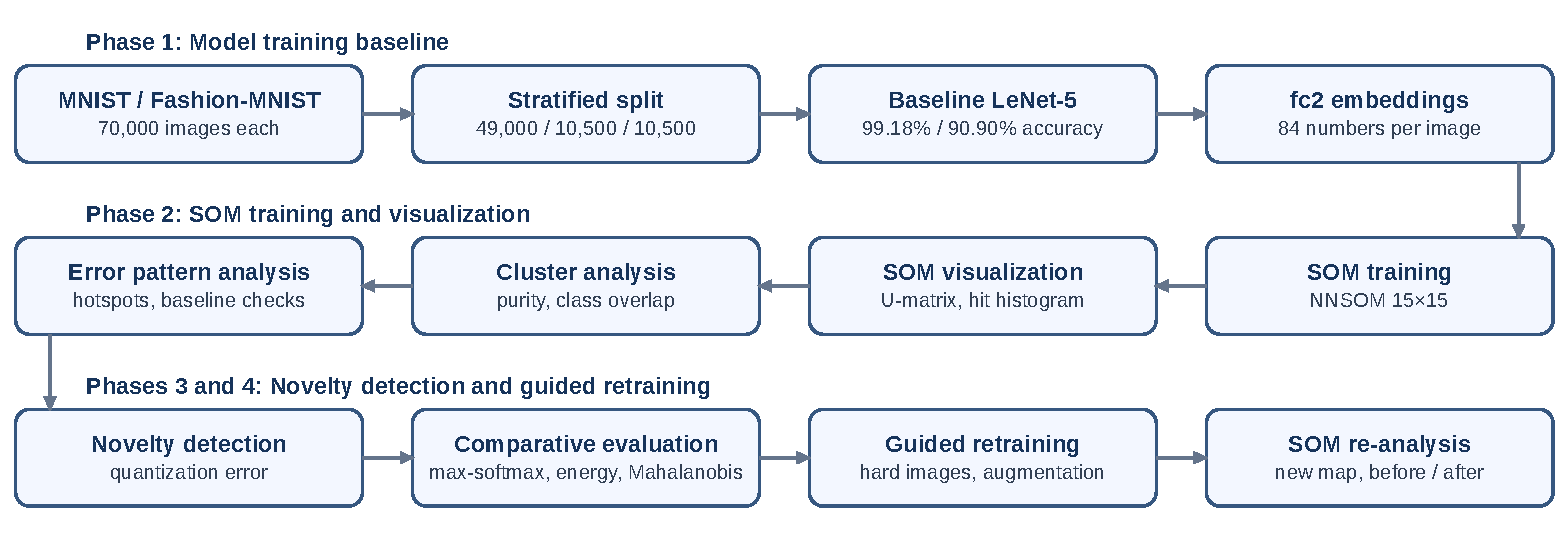
\includegraphics[width=\linewidth]{diagrams/project_pipeline.pdf}
\caption{The project pipeline, run unchanged on both datasets: the baseline CNN (Phase 1), the SOM (Phase 2), novelty detection (Phase 3) and guided retraining with a new SOM (Phase 4). Accuracies are the baseline test accuracies on MNIST and Fashion-MNIST.}
\label{fig:pipeline}
\end{figure}

\subsection{Datasets and preparation}

\begin{itemize}
  \item \textbf{MNIST:} 70,000 greyscale $28\times28$ images of handwritten digits in 10 classes.
  \item \textbf{Fashion-MNIST:} 70,000 greyscale $28\times28$ images of clothing in 10 classes (T-shirt/top, Trouser, Pullover, Dress, Coat, Sandal, Shirt, Sneaker, Bag, Ankle boot).
  \item \textbf{Split:} as specified in the proposal, each dataset is split once into 70\% training (49,000 images), 15\% validation (10,500) and 15\% test (10,500), stratified by class with a fixed random seed. Pixel values are scaled to $[0,1]$.
  \item \textbf{Out-of-distribution data:} the 26,032 images of the SVHN test set~\cite{netzer2011reading} (photographs of house numbers), converted to greyscale and resized to $28\times28$. The same images are used for both datasets.
\end{itemize}

\subsection{Phase 1: Model Training Baseline}

\begin{itemize}
  \item LeNet-5~\cite{lecun1998gradient} is trained with Adam~\cite{kingma2015adam} (learning rate 0.001, weight decay 0.0001, learning rate multiplied by 0.1 every 10 epochs, batch size 64, 20 epochs, seed 42). The checkpoint with the highest validation accuracy is retained. LeNet-5 is the only network architecture used in this study: the project proposal specifies it for MNIST, and the same recipe was kept for Fashion-MNIST.
  \item Evaluation metrics are accuracy with a 95\% Wilson confidence interval~\cite{wilson1927probable}, per-class precision, recall and F1, macro-F1, and the confusion matrix.
  \item For every image in every split, the 84 activations of the penultimate fully connected layer (fc2) are stored as the embedding, together with the label, prediction and confidence. The embeddings are rescaled to $[-1,1]$ using statistics from the training set only.
\end{itemize}

\subsection{Phase 2: SOM Training and Visualization}

\textbf{SOM principle.} A SOM is a competitive network consisting of a layer of neurons arranged on a grid, each with a weight vector of the same dimension as the input~\cite{kohonen1990som,hagan2014nnd_ch16}. For each input, the neuron whose weight vector is closest wins the competition. The winner and its neighbours on the grid then move their weights towards the input. Because neighbouring neurons are updated together, nearby cells come to represent similar inputs, and the grid becomes a two-dimensional summary of the data. NNSOM uses the batch version of this rule~\cite{hagan2014nnd_ch26}, which requires no learning rate: after each pass over the data, each weight vector is replaced by a weighted average of the embeddings whose winning neurons lie in its neighbourhood. Figure~\ref{fig:som_explained} illustrates these steps.

\begin{figure}[H]
\centering
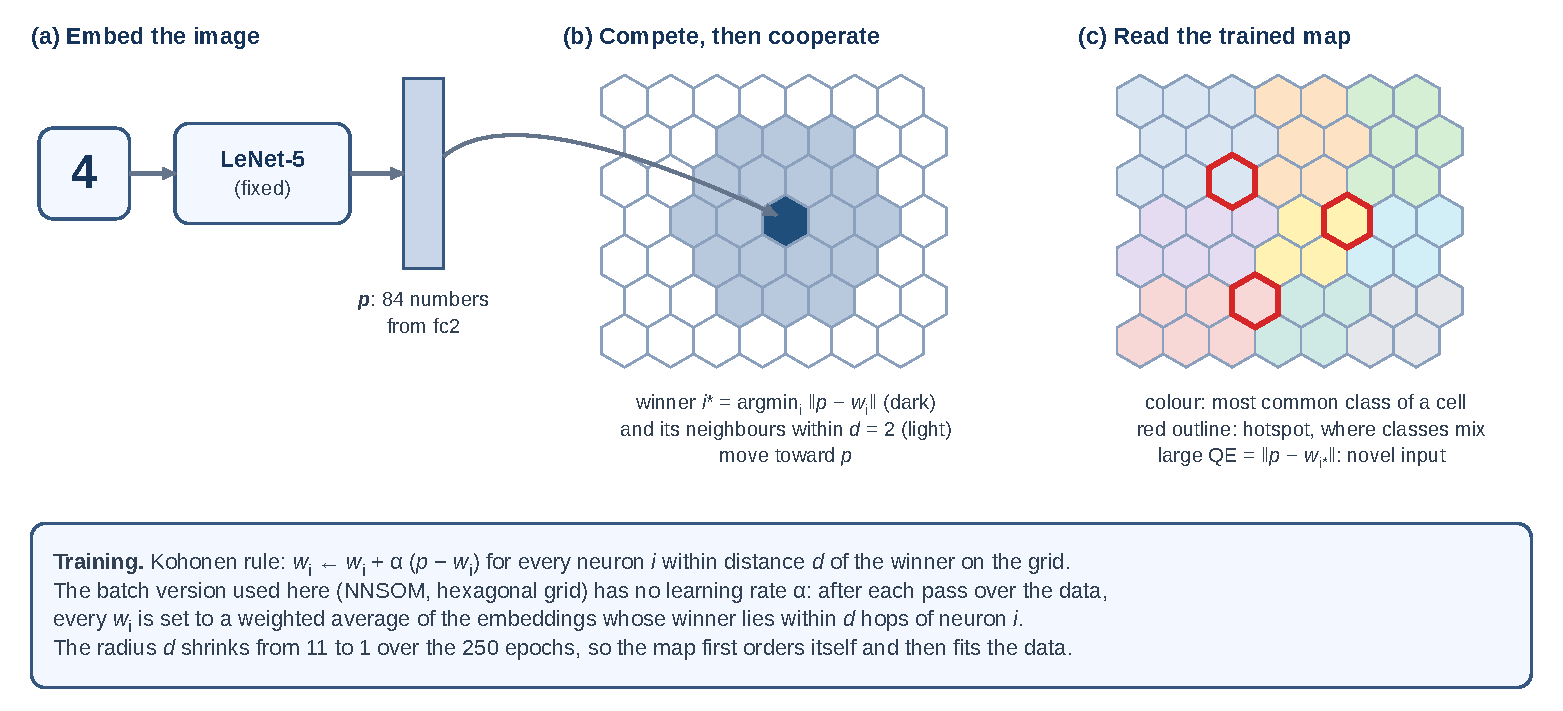
\includegraphics[width=\linewidth]{diagrams/som_explained.pdf}
\caption{How the self-organizing map works in this project. (a)~Each image (here an MNIST digit) is turned into an 84-number embedding by the fixed CNN. (b)~The neuron whose weight vector is closest wins, and the winner and its grid neighbours move toward the embedding. (c)~After training, each cell is labelled by its images: their most common class, how mixed the classes are, and how often the CNN is wrong there (hotspots). An image far from its best cell (large quantization error, QE) is unlike the training data. The grids are schematic; the real maps have 15$\times$15 hexagonal cells. Adapted from~\cite{hagan2014nnd_ch16,hagan2014nnd_ch26}.}
\label{fig:som_explained}
\end{figure}

\begin{itemize}
  \item \textbf{Map training.} A hexagonal $15\times15$ SOM (225 cells) is trained with NNSOM's batch rule on the 49,000 training embeddings for 250 epochs, with the neighbourhood radius decreasing from 11 to 1 (seed 42). Each image is assigned to its best-matching unit (BMU), the cell with the closest weight vector. Map quality is measured by the quantization error (QE, the mean distance between an image and its BMU) and the topographic error (TE1, the proportion of images whose two closest cells are not adjacent on the grid).
  \item \textbf{Grid size.} Grids of $10\times10$, $15\times15$ and $20\times20$ were compared with a pre-specified procedure: ten maps were trained per grid, and the error rate of each cell, estimated on one half of the validation set, was used to predict the errors on the other half (AUROC), over 200 random splits. Retraining all maps of the MNIST comparison with the final code reproduced the same choices and verdicts. A 20-trial Optuna~\cite{akiba2019optuna} search per grid (scored on validation QE and TE1 only, followed by 5 new seeds for the best setting) checked the initial radius and the number of epochs; the headline map was fixed regardless of its outcome.
  \item \textbf{Feature layer.} As the proposal requires, SOMs trained on the earlier fc1 layer (120 dimensions) and on fc2 were compared using 5 SOM seeds each. Three statements were fixed in advance: which layer locates the errors better (the primary statement), which yields purer cells, and which detects SVHN better.
  \item \textbf{Cluster analysis.} Each image is assigned to its BMU. For each cell we compute the purity (the proportion of its images that belong to its majority class) and the class entropy, and we compare the overall purity with 1,000 random label permutations. Confusions are overlaid on the map.
  \item \textbf{Error hotspots.} Cells are ranked by the lower bound of the 95\% Wilson interval of their error rate, and the top 5\% (11 cells) are designated as hotspots. Hotspots are selected on one half of the validation set and evaluated on the other half using the concentration ratio, defined as the proportion of errors in the hotspots divided by the proportion of images in the hotspots. This is repeated over 200 random splits and compared with 200 permutations of the error labels.
  \item \textbf{Baselines.} The same error-localisation test is applied to k-means clustering with 225 clusters, to the class impurity of the 15 nearest training embeddings, and to the network's maximum softmax probability~\cite{hendrycks2017baseline}.
\end{itemize}

\subsection{Phase 3: Novelty Detection}

\begin{itemize}
  \item \textbf{Far novelty.} The 10,500 validation images of each dataset serve as in-distribution (normal) data, and the 26,032 SVHN test images serve as out-of-distribution (novel) data.
  \item \textbf{SOM scores.} We use two scores: the quantization error (the distance to the BMU) and the U-matrix score (the mean distance between the BMU and its neighbouring cells). The detection threshold is the 95th percentile of the training QE (1.569 on MNIST and 1.4215 on Fashion-MNIST), fixed before any novel image was scored.
  \item \textbf{Comparison methods.} On the same embeddings we compute the maximum softmax probability, the energy score~\cite{liu2020energy}, the Mahalanobis distance~\cite{lee2018mahalanobis}, the nearest-neighbour distance~\cite{sun2022knn}, Isolation Forest~\cite{liu2008isolation}, the One-Class SVM~\cite{scholkopf2001support} and an autoencoder~\cite{sakurada2014autoencoder}, together with a random score as a control.
  \item \textbf{Near novelty.} Because SVHN differs strongly from both datasets, it provides an easy test. For a harder test we follow the open-set protocol~\cite{neal2018open}. In each of 5 class splits, drawn once at random and fixed before any run, a new LeNet-5 and a new $15\times15$ SOM are trained on 6 known classes only, and the validation images of the remaining 4 classes serve as novel data. The maximum softmax probability is a strong baseline in this setting~\cite{vaze2022openset}. Four hypotheses were specified in advance: (H1) the SOM detects the unseen classes; (H2, primary) it outperforms the maximum softmax probability; (H3) it is no more than 0.01 AUROC worse than the maximum softmax probability, energy or Mahalanobis distance; (H4) it outperforms the nearest-neighbour distance. Each is tested with a 95\% $t$-interval over the five splits and is classified as supported, contradicted or inconclusive.
  \item \textbf{Metrics.} We report the AUROC~\cite{fawcett2006roc}, the AUPR with novel images as the positive class~\cite{saito2015pr}, the false-positive rate at 95\% true-positive rate, and paired bootstrap intervals (2,000 resamples).
\end{itemize}

\subsection{Phase 4: Guided Retraining}

\begin{itemize}
  \item \textbf{Hard-example pool.} A training image is considered hard if its cell is one of the 11 hotspots, if its cell's purity is below 0.95, or if its distance to its BMU exceeds the 95th percentile. Two control pools of the same size and class composition are formed: randomly selected images, and the least-confident images (lowest maximum softmax probability).
  \item \textbf{Curriculum learning.} Training starts with the easy images and 10\% of the hard pool, and a further 10\% of the pool is added every 5 epochs, following the pacing function suggested in the proposal.
  \item \textbf{Targeted augmentation.} Three augmented copies (small rotation, translation, scaling and shear) of every pool image are added to the training set. Before any training, the augmentation ranges must pass a check: the baseline network may lose at most 2 percentage points of validation accuracy on augmented images. Gradually paced variants are also evaluated.
  \item \textbf{Training and evaluation.} Each arm is retrained from scratch with the Phase 1 recipe for seeds 1 to 5, using the same seeds in every arm. The test set is evaluated once, after the success criteria (Table~\ref{tab:criteria}) and a macro-F1 guard had been recorded and time-stamped with a SHA-256 hash. Differences between arms are assessed with paired bootstrap intervals over the test images.
  \item \textbf{SOM re-analysis.} Embeddings are extracted from each retrained network and a new $15\times15$ SOM is trained on them (normal training, SOM-guided and random augmentation; 5 seeds each). The new maps are evaluated on the validation set in terms of purity, topographic error and the error rate in their 11 worst cells. Each retrained network is also re-evaluated on SVHN.
  \item \textbf{End-to-end comparison.} In the first path, a test image is classified by the normally trained CNN, giving the confusion matrix CF1. In the second path, it is classified by the CNN retrained with SOM-guided augmentation, giving CF2. Both are averaged over the same 5 seeds.
\end{itemize}

\begin{figure}[H]
\centering
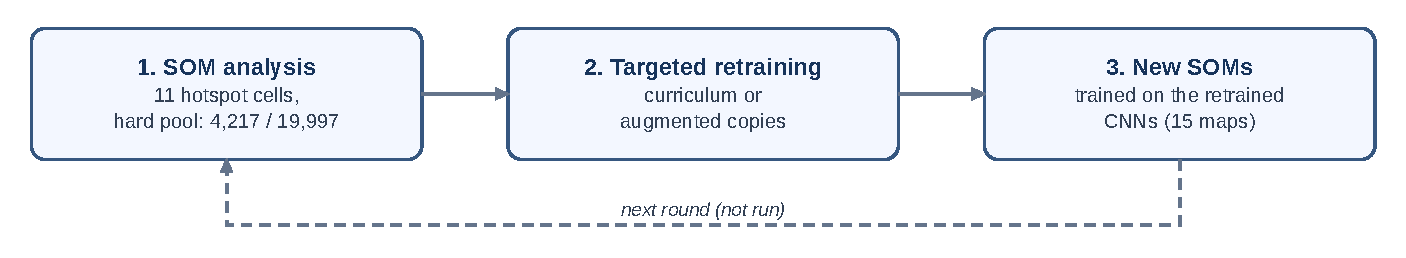
\includegraphics[width=0.9\linewidth]{diagrams/guided_retraining_loop.pdf}
\caption{The feedback loop of Phase 4: SOM analysis $\rightarrow$ targeted retraining $\rightarrow$ new SOM structure. The hard pool holds 4,217 training images on MNIST and 19,997 on Fashion-MNIST. The dashed arrow marks a next round, which we did not run.}
\label{fig:loop}
\end{figure}

\begin{figure}[H]
\centering
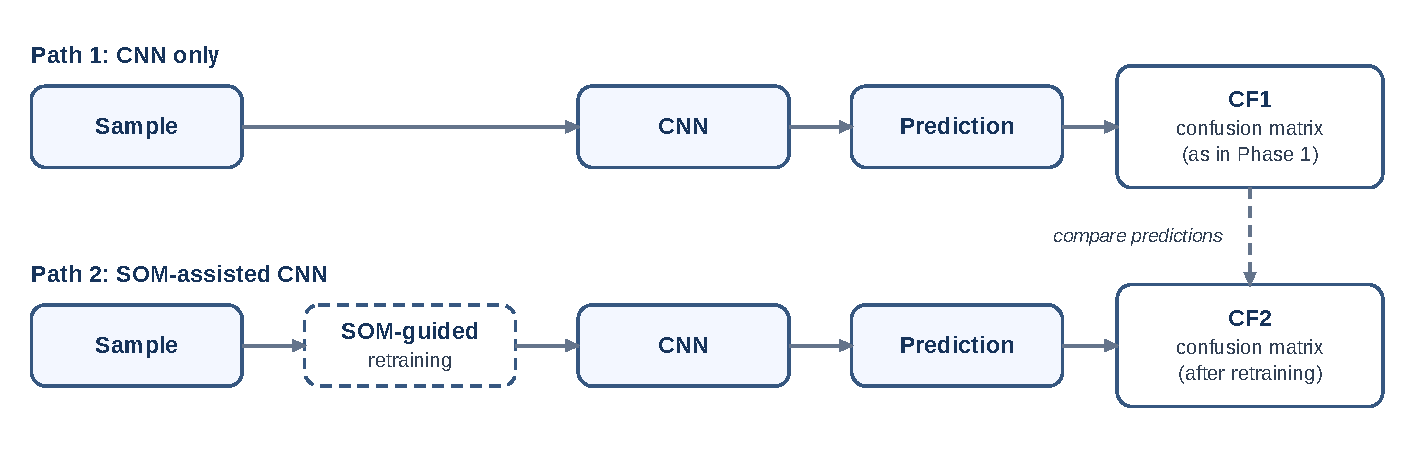
\includegraphics[width=0.9\linewidth]{diagrams/end_to_end_comparison.pdf}
\caption{End-to-end comparison: sample $\rightarrow$ CNN $\rightarrow$ prediction (CF1) against sample $\rightarrow$ SOM-guided retraining $\rightarrow$ CNN $\rightarrow$ prediction (CF2), on the same test samples. The dashed box is the step that uses the SOM.}
\label{fig:endtoend}
\end{figure}

For a fair end-to-end comparison, CF1 is computed not from the single Phase 1 network but from the five-seed average of the normally retrained arm (99.11\% on MNIST and 90.66\% on Fashion-MNIST, compared with 99.18\% and 90.90\% for the single Phase 1 networks). Both paths use the same recipe, data and seeds, so any difference can be attributed to the SOM guidance.

% ------------------------------------------------------------------------------------------------------------------------
\section{Results and Discussion}\label{sec:results}

This section first describes the experimental protocol, then presents the results for both datasets in tables, and finally shows the corresponding figures.

\subsection{Experimentation protocol}

\begin{itemize}
  \item \textbf{Pre-registration.} Success criteria, thresholds, numbers of splits and permutations, and random seeds were recorded in a protocol before the corresponding results were seen; for Phase 4, the protocol was time-stamped with a SHA-256 hash before the test set was opened. The Fashion-MNIST protocol reproduced the MNIST design and was written before any Fashion-MNIST data were loaded. Changes required by the dataset followed rules that were recorded before the next run.
  \item \textbf{Leakage control.} The scaler, the SOM, k-means, the nearest-neighbour reference set, the novelty detectors and the QE threshold are fitted on training embeddings only, and all Phase 2 and Phase 3 statistics are computed on validation images. The test set was used only to evaluate the baseline network and once in the final Phase 4 evaluation; no setting was selected on it. SVHN images were used only for scoring. In the near-novelty experiment, the held-out classes were never used for training, checkpoint selection, fitting or threshold setting. Because the validation set was also used to select the network checkpoint, it is not entirely independent of model development.
  \item \textbf{Uncertainty.} Accuracies are reported with Wilson intervals; differences with paired bootstrap intervals over images (2,000 resamples) or $t$-intervals over 5 seeds; and map statistics are compared with permutation controls (1,000 permutations for purity and 200 for hotspots).
  \item \textbf{Fair comparisons.} All retraining arms use the same data, training recipe, number of added images and seeds. Criteria that were not met are reported as such, and no criterion was changed after the test evaluation.
  \item \textbf{Exploratory analyses.} Comparisons designed after earlier results were known (the equal-budget baseline comparison, the classical novelty detectors and the embedding-length diagnostics) are labelled as exploratory.
  \item \textbf{Reproducibility.} Each run has a unique identifier and records the SHA-256 hashes of its inputs; completed runs are never overwritten.
\end{itemize}

\subsection{Data tables}

\subsubsection*{Phase 1: baseline networks}

\begin{table}[H]
\centering
\caption{Baseline LeNet-5 on Both Datasets}
\label{tab:baseline}
\renewcommand{\arraystretch}{1.12}
\small
\begin{tabular}{|L{0.36\textwidth}|C{0.26\textwidth}|C{0.26\textwidth}|}
\hline
\textbf{Measure} & \textbf{MNIST} & \textbf{Fashion-MNIST} \\ \hline
Test accuracy (95\% Wilson interval) & 99.18\% (98.99--99.34) & 90.90\% (90.33--91.43) \\ \hline
Macro-F1 (test) & 0.9918 & 0.9089 \\ \hline
Mistakes: test / validation / training & 86 / 92 / 29 & 956 / 876 / 3,311 \\ \hline
Mean confidence when right / wrong (validation) & 0.997 / 0.833 & 0.942 / 0.686 \\ \hline
Most common confusions & 5$\rightarrow$0, 9$\rightarrow$4, 4$\rightarrow$9 & Shirt$\leftrightarrow$T-shirt/top, Pullover$\rightarrow$Coat \\ \hline
\end{tabular}

\par\vspace{3pt}
{\footnotesize\raggedright\noindent On Fashion-MNIST, confusions among T-shirt/top, Pullover, Coat and Shirt make up 638 of the 956 test mistakes (67\%), and Shirt is the weakest class (F1 0.746).\par}
\end{table}

Fashion-MNIST produces about ten times as many errors as MNIST, and the network is often wrong with high confidence. These errors are concentrated in a few groups of visually similar classes, which is the pattern examined on the map in Phase 2.

\subsubsection*{Phase 2: map structure and error concentration}

\begin{table}[H]
\centering
\caption{SOM Structure and Error Concentration}
\label{tab:som}
\renewcommand{\arraystretch}{1.12}
\small
\begin{tabular}{|L{0.50\textwidth}|C{0.18\textwidth}|C{0.18\textwidth}|}
\hline
\textbf{Measure (validation images, 15$\times$15 map)} & \textbf{MNIST} & \textbf{Fashion-MNIST} \\ \hline
Quantization error (training) & 1.041 (1.039) & 0.899 (0.915) \\ \hline
Topological error TE1 & 6.18\% & 5.37\% \\ \hline
Purity (with shuffled labels) & 98.2\% (17.4\%) & 89.3\% (17.3\%) \\ \hline
Cells with purity below 95\% & 44 & 121 \\ \hline
Hotspot concentration ratio, held out (95\% range) & 11.1 (6.1--17.6) & 3.9 (3.2--4.4) \\ \hline
Chance level of the ratio & about 1.0 & about 1.0 \\ \hline
Spearman, cell error rate vs.\ purity & $-0.810$ & $-0.946$ \\ \hline
Spearman, cell error rate vs.\ class mix (entropy) & $+0.816$ & $+0.956$ \\ \hline
Cells holding each of the top three confusions & 4 to 5 & 24 to 27 \\ \hline
Mean distance to cell, wrong / correct images & 1.349 / 0.960 & 0.994 / 0.840 \\ \hline
\end{tabular}

\par\vspace{3pt}
{\footnotesize\raggedright\noindent All label-shuffle tests give $p=0.001$ (purity) or $p=0.005$ (hotspots, Spearman). The concentration ratio cannot exceed one divided by the error rate (about 114 on MNIST, about 12 on Fashion-MNIST), so the two ratios are not comparable.\par}
\end{table}

\begin{itemize}
  \item \textbf{Class structure.} On both maps the classes occupy distinct regions, well beyond chance. On Fashion-MNIST, footwear, trousers and bags form almost pure regions, whereas the upper-body garments share one large mixed region.
  \item \textbf{Error concentration.} Errors concentrate where classes overlap, on both datasets and also on the $10\times10$ and $20\times20$ maps (ratios of 10.5 and 13.4 on MNIST, and 3.81 and 3.81 on Fashion-MNIST). The error rate of a cell is strongly correlated with its class mixture.
  \item \textbf{Nature of the errors.} On MNIST, each frequent confusion (4 predicted as 9, 5 as 0, and 9 as 4) is located in four or five cells, mostly among the cells of the predicted digit; the hotspot images suggest digits that share strokes (4 and 9, 7 and 9, 5, 6 and 8) and some unusual handwriting. On Fashion-MNIST, each frequent confusion spreads over 24 to 27 cells, and every hotspot mixes upper-body garments (Coat with Shirt or Dress, Pullover with Coat, Shirt with T-shirt/top). At $28\times28$ pixels, a collar, buttons or sleeve length occupy only a few pixels, so entire classes overlap. These interpretations of the hotspot images are hypotheses rather than tested results.
\end{itemize}

\begin{table}[H]
\centering
\caption{Ablations: Grid Size, Settings and Feature Layer}
\label{tab:ablation}
\renewcommand{\arraystretch}{1.12}
\footnotesize
\begin{tabular}{|L{0.40\textwidth}|C{0.25\textwidth}|C{0.25\textwidth}|}
\hline
\textbf{Check} & \textbf{MNIST} & \textbf{Fashion-MNIST} \\ \hline
QE / TE1 for 10$\times$10, 15$\times$15, 20$\times$20 (mean of 10 maps) & 1.21, 1.06, 0.98 / 4.8, 6.6, 7.7\% & 1.05, 0.91, 0.84 / 4.8, 6.3, 7.7\% \\ \hline
Mistake AUROC, 20$\times$20 minus 15$\times$15 & $+0.001$ ($-0.100$, $+0.089$): inconclusive & $-0.042$ ($-0.077$, $-0.008$): 15$\times$15 better \\ \hline
Optuna setting minus fixed setting, 15$\times$15: QE / TE1 & $+0.005$ ($-0.003$, $+0.013$) / $-0.14$ ($-0.81$, $+0.53$): not better; map unchanged & $-0.014$ ($-0.024$, $-0.004$) / $+2.4$ ($+1.6$, $+3.2$): not better on both; map unchanged \\ \hline
Mistake AUROC, fc1 vs fc2 map (main) & 0.622 vs 0.685, $-0.062$ ($-0.073$, $-0.052$): fc2 better & 0.760 vs 0.815, $-0.055$ ($-0.066$, $-0.043$): fc2 better \\ \hline
Purity, fc1 vs fc2 map & 0.961 vs 0.982, $-0.021$ ($-0.022$, $-0.020$): fc2 better & 0.842 vs 0.890, $-0.048$ ($-0.051$, $-0.045$): fc2 better \\ \hline
SVHN QE AUROC, fc1 vs fc2 map & 0.986 vs 0.981, $+0.005$ ($+0.003$, $+0.006$): fc1 better & 0.902 vs 0.815, $+0.087$ ($+0.027$, $+0.148$): fc1 better \\ \hline
\end{tabular}

\par\vspace{3pt}
{\footnotesize\raggedright\noindent Grid differences are 95\% ranges over 200 half-splits; the Optuna and feature-layer comparisons are 95\% $t$-intervals over 5 SOM seeds. With 876 mistakes instead of 92, the Fashion-MNIST grid ranges are about three times narrower. On MNIST, tuning found a better 10$\times$10 setting, which is used only for the robustness check.\par}
\end{table}

\begin{table}[H]
\centering
\caption{Error Detection by the SOM and Simple Baselines}
\label{tab:baselines}
\renewcommand{\arraystretch}{1.12}
\footnotesize
\begin{tabular}{|L{0.28\textwidth}|C{0.13\textwidth}|C{0.13\textwidth}|C{0.13\textwidth}|C{0.13\textwidth}|}
\hline
 & \multicolumn{2}{c|}{\textbf{MNIST (92 mistakes)}} & \multicolumn{2}{c|}{\textbf{Fashion-MNIST (876 mistakes)}} \\ \hline
\textbf{Method} & \textbf{AUROC} & \textbf{Mistakes caught} & \textbf{AUROC} & \textbf{Mistakes caught} \\ \hline
SOM cell error rate (15$\times$15) & 0.685 & 18.1\% & 0.811 & 13.7\% \\ \hline
k-means cell error rate (225) & 0.693 & 20.4\%$^*$ & 0.812 & 15.8\%$^*$ \\ \hline
15-nearest-neighbour impurity & 0.874 & 48.7\% & 0.876 & 21.1\% \\ \hline
Network max-softmax confidence & \textbf{0.981} & \textbf{53.3\%} & \textbf{0.906} & \textbf{21.9\%} \\ \hline
\end{tabular}

\par\vspace{3pt}
{\footnotesize\raggedright\noindent ``Mistakes caught'': share of mistakes among the images flagged when every method flags the same share as the SOM's hotspots (MNIST 1.6\%, Fashion-MNIST 3.5\%); $^*$k-means flags its own hotspot share (3.8\% and 4.0\%). The same-budget check is exploratory.\par}
\end{table}

\textbf{The SOM is not the best error detector.} On both datasets, k-means clustering locates the errors as well as the SOM, and the network's own confidence performs best. The gap is smaller on Fashion-MNIST, where the network is more often wrong with high confidence.

\subsubsection*{Phase 3: novelty detection}

\begin{table}[H]
\centering
\caption{Far Novelty Detection Against SVHN}
\label{tab:far}
\renewcommand{\arraystretch}{1.12}
\footnotesize
\begin{tabular}{|L{0.38\textwidth}|C{0.10\textwidth}|C{0.10\textwidth}|C{0.10\textwidth}|C{0.10\textwidth}|}
\hline
 & \multicolumn{2}{c|}{\textbf{MNIST vs SVHN}} & \multicolumn{2}{c|}{\textbf{Fashion-MNIST vs SVHN}} \\ \hline
\textbf{Novelty score} & \textbf{AUROC} & \textbf{FPR@95} & \textbf{AUROC} & \textbf{FPR@95} \\ \hline
Energy & \textbf{0.9998} & 0.0004 & \textbf{0.982} & 0.063 \\ \hline
Maximum softmax probability & 0.9985 & 0.008 & 0.884 & 0.307 \\ \hline
SOM quantization error (QE) & 0.981 & 0.045 & 0.789 & 0.420 \\ \hline
Nearest-neighbour distance ($k=5$) & 0.977 & 0.059 & 0.864 & 0.314 \\ \hline
SOM U-matrix score & 0.970 & 0.070 & 0.812 & 0.253 \\ \hline
One-Class SVM & 0.960 & 0.179 & 0.734 & 0.634 \\ \hline
Mahalanobis distance & 0.776 & 0.313 & 0.713 & 0.454 \\ \hline
Isolation Forest & 0.238 & 0.872 & 0.266 & 0.934 \\ \hline
Autoencoder (raw inputs) & 0.008 & 0.9999 & 0.583 & 0.744 \\ \hline
SVHN caught by the fixed QE alarm (normal flagged) & \multicolumn{2}{c|}{96.2\% (5.1\%)} & \multicolumn{2}{c|}{3.0\% (5.1\%)} \\ \hline
\end{tabular}

\par\vspace{3pt}
{\footnotesize\raggedright\noindent 10,500 validation images (normal) against 26,032 SVHN test images (novel), one network and one map per dataset. FPR@95: share of normal images flagged when 95\% of SVHN is caught. A random score gives AUROC 0.505; label shuffles give 0.500. The classical detectors are exploratory.\par}
\end{table}

\begin{itemize}
  \item \textbf{Detection of SVHN.} The SOM detects SVHN on both datasets, with QE well above chance: strongly on MNIST and weakly on Fashion-MNIST. The energy score and the maximum softmax probability perform better on both. The difference between QE and the maximum softmax probability is $-0.017$ AUROC ($-0.019$ to $-0.015$) on MNIST and $-0.094$ on Fashion-MNIST.
  \item \textbf{Paired comparisons.} On MNIST, QE is slightly better than the nearest-neighbour distance ($+0.005$, $+0.002$ to $+0.007$), the U-matrix score ($+0.011$) and the Mahalanobis distance ($+0.205$), but worse than the energy score ($-0.019$, $-0.021$ to $-0.017$). On Fashion-MNIST, QE is worse than the energy score ($-0.193$), the maximum softmax probability, the nearest-neighbour distance ($-0.074$) and the U-matrix score ($-0.022$), and better only than the Mahalanobis distance ($+0.076$). On both datasets the SOM detects SVHN but is not competitive with the strongest baseline.
  \item \textbf{Fixed threshold.} The QE threshold works on MNIST but not on Fashion-MNIST, where it flags a smaller proportion of SVHN images than of normal images.
  \item \textbf{Embedding length.} SVHN embeddings have a much smaller norm (mean length 5.8 against 40.3 on MNIST, and 8.5 against 20.7 on Fashion-MNIST). On MNIST, QE is strongly correlated with length (Spearman $-0.83$), which favours it; on Fashion-MNIST the correlation is weak ($-0.29$), while length alone separates SVHN almost perfectly (0.995).
  \item \textbf{Inverted detectors.} Isolation Forest rates SVHN as more normal than the in-distribution data on both datasets, consistent with previous findings for models of normal data~\cite{nalisnick2019deep}. The autoencoder is sensitive to input scaling (0.979 on MNIST with standardised inputs).
  \item \textbf{Location of SVHN on the map.} On MNIST, all SVHN images fall in 28 of the 225 cells, and a single cell, mostly containing the digit 4, receives 86.5\% of them. On Fashion-MNIST they fall in 42 cells, 91\% of them in cells whose majority class is Bag.
\end{itemize}

\begin{table}[H]
\centering
\caption{Near Novelty Detection on Held-Out Classes}
\label{tab:near}
\renewcommand{\arraystretch}{1.12}
\footnotesize
\begin{tabular}{|L{0.25\textwidth}|C{0.30\textwidth}|C{0.30\textwidth}|}
\hline
\textbf{Mean AUROC over 5 class splits} & \textbf{MNIST (held-out digits)} & \textbf{Fashion-MNIST (held-out classes)} \\ \hline
SOM quantization error & 0.912 & 0.794 \\ \hline
Maximum softmax probability & 0.944 & 0.749 \\ \hline
Energy & 0.927 & 0.783 \\ \hline
Mahalanobis distance & 0.927 & 0.823 \\ \hline
Nearest-neighbour distance & \textbf{0.966} & \textbf{0.842} \\ \hline
QE minus max-softmax (95\% interval) & $-0.032$ ($-0.095$, $+0.032$): inconclusive & $+0.046$ ($+0.034$, $+0.057$): \textbf{QE better} \\ \hline
QE minus nearest neighbour (95\% interval) & $-0.054$ ($-0.084$, $-0.024$) & $-0.048$ ($-0.071$, $-0.026$) \\ \hline
\end{tabular}

\par\vspace{3pt}
{\footnotesize\raggedright\noindent 4 classes held out of training in each of 5 splits, with a new network and map per split. Statements fixed before the run; intervals are $t$-intervals over the 5 splits.\par}
\end{table}

\begin{itemize}
  \item \textbf{H1 supported on both datasets.} The split networks reach 99.1--99.4\% (MNIST) and 92.8--96.6\% (Fashion-MNIST) accuracy on their known classes, and QE detects the unseen classes in every split (AUROC 0.860 to 0.957 and 0.739 to 0.831; label permutation gives 0.500).
  \item \textbf{No length effect.} Embedding length alone yields only 0.63 to 0.89 (MNIST) and 0.687 on average (Fashion-MNIST), below QE.
  \item \textbf{H2 and H3.} On MNIST, QE is lower than the maximum softmax probability in 4 of 5 splits (H2 inconclusive), and it is not shown to be within 0.01 of the maximum softmax probability, energy or Mahalanobis distance (H3 inconclusive). On Fashion-MNIST, H2 is supported; H3 is supported for the maximum softmax probability and inconclusive for energy and Mahalanobis distance.
  \item \textbf{H4 contradicted on both datasets:} the nearest-neighbour distance outperforms QE in every split.
  \item \textbf{Location of unseen classes.} 90\% of the novel images fall in 33 to 55 cells (MNIST) and 71 to 97 cells (Fashion-MNIST), whereas 90\% of the normal images require 166 to 174 and 170 to 174 cells.
\end{itemize}

\textbf{On unseen classes, the SOM outperforms the network's confidence on Fashion-MNIST} in all 5 splits. Because clothing classes are visually similar, the network often assigns an unseen class to a known class with high confidence, while the map still places it away from the known prototypes. On MNIST this comparison is inconclusive. On both datasets, the nearest-neighbour distance outperforms the SOM, indicating that the 225 cells discard some information contained in the training embeddings.

\subsubsection*{Phase 4: guided retraining}

\begin{table}[H]
\centering
\caption{Phase 4 Settings}
\label{tab:p4settings}
\renewcommand{\arraystretch}{1.12}
\footnotesize
\begin{tabular}{|L{0.36\textwidth}|C{0.25\textwidth}|C{0.25\textwidth}|}
\hline
\textbf{Setting} & \textbf{MNIST} & \textbf{Fashion-MNIST} \\ \hline
SOM hard pool & 4,217 images (8.6\%) & 19,997 images (40.8\%) \\ \hline
Augmentation ranges that passed the check & rotation 10$^\circ$, shift 1 px, zoom 0.9--1.1, shear 8$^\circ$ & rotation 2.5$^\circ$, shift 0.25 px, zoom 0.975--1.025, shear 2$^\circ$ \\ \hline
Validation accuracy on altered images (original) & 98.21\% (99.12\%) & 90.46\% (91.66\%) \\ \hline
Macro-F1 guard & 0.0016 & 0.0033 \\ \hline
Test images on the hotspots & 146 & 422 \\ \hline
\end{tabular}

\par\vspace{3pt}
{\footnotesize\raggedright\noindent The first augmentation ranges failed the check on both datasets (MNIST with 2-pixel shifts; Fashion-MNIST with MNIST's ranges and with them halved), and were reduced by rules written down before the next check. Clothing fills the frame, so turns and zooms cut off the sleeves and hems that separate similar garments.\par}
\end{table}

\begin{table}[H]
\centering
\caption{Baseline and Post-Retraining Test Accuracy}
\label{tab:retraining}
\renewcommand{\arraystretch}{1.12}
\footnotesize
\begin{tabular}{|l|C{0.11\textwidth}|C{0.11\textwidth}|C{0.11\textwidth}|C{0.11\textwidth}|}
\hline
 & \multicolumn{2}{c|}{\textbf{MNIST}} & \multicolumn{2}{c|}{\textbf{Fashion-MNIST}} \\ \hline
\textbf{Arm (mean of 5 seeds)} & \textbf{Accuracy} & \textbf{Hotspot error} & \textbf{Accuracy} & \textbf{Hotspot error} \\ \hline
Normal training (CF1) & 99.11\% & 11.4\% & 90.66\% & 36.0\% \\ \hline
Augmentation, random images & 99.18\% & 10.3\% & 90.60\% & 35.0\% \\ \hline
Augmentation, least-confident images & 99.25\% & 8.5\% & 90.57\% & 35.2\% \\ \hline
Augmentation, SOM-chosen images (CF2) & 99.21\% & \textbf{7.8\%} & 90.62\% & 34.0\% \\ \hline
Curriculum, SOM order & 98.66\% & 21.4\% & 87.37\% & 51.8\% \\ \hline
Curriculum, random order & 99.07\% & 12.2\% & 89.15\% & 42.1\% \\ \hline
\end{tabular}

\par\vspace{3pt}
{\footnotesize\raggedright\noindent Hotspot error is measured on the test images that fall on the 11 hotspot cells of the original map. The single Phase 1 networks scored 99.18\% and 90.90\%.\par}
\end{table}

\begin{table}[H]
\centering
\caption{Phase 4 Success Criteria}
\label{tab:criteria}
\renewcommand{\arraystretch}{1.12}
\footnotesize
\begin{tabular}{|L{0.40\textwidth}|C{0.24\textwidth}|C{0.24\textwidth}|}
\hline
\textbf{Success criterion (fixed before the test)} & \textbf{MNIST} & \textbf{Fashion-MNIST} \\ \hline
A1 (primary): SOM copies beat random copies on hotspot error & $-2.47$ ($-4.52$, $-0.68$): \textbf{met} & $-1.04$ ($-3.22$, $+1.14$): not met \\ \hline
A2: SOM copies beat normal training on hotspot error & $-3.56$ ($-5.75$, $-1.37$): \textbf{met} & $-1.99$ ($-4.79$, $+0.71$): not met \\ \hline
A3: no damage outside the hotspots (upper end $\le 0.2$) & $-0.05$ ($-0.13$, $+0.02$): \textbf{met} & $+0.13$ ($-0.12$, $+0.37$): not met \\ \hline
C1: SOM curriculum beats normal training & $+0.45$: worse & $+3.29$: worse \\ \hline
C2: SOM curriculum beats random curriculum on hotspots & $+9.18$: worse & $+9.76$: worse \\ \hline
\end{tabular}

\par\vspace{3pt}
{\footnotesize\raggedright\noindent Difference in test error (percentage points, first arm minus second) with the 95\% paired bootstrap interval. C1, C2, A1 and A2 also require the macro-F1 guard to hold.\par}
\end{table}

\begin{itemize}
  \item \textbf{MNIST: SOM-guided augmentation reduced the errors in the hotspots}, by about 5 of the 146 hotspot images, without increasing the error elsewhere. Random and least-confident augmentation also slightly reduced the overall error, so only the hotspot improvement is specific to the SOM.
  \item \textbf{Fashion-MNIST: no significant improvement.} The hard pool contains 41\% of the training images and is therefore much less selective, and the augmentation ranges had to be four times smaller than on MNIST.
  \item \textbf{The SOM is not a better selector than confidence.} On both datasets, SOM-selected and least-confident images cannot be distinguished.
  \item \textbf{Curriculum learning degraded accuracy on both datasets}, more strongly on Fashion-MNIST. Because the schedule never uses more than 40\% of the hard pool, the hardest 60\% is never trained on; this corresponds to about 5\% of all training images on MNIST and about a quarter on Fashion-MNIST.
  \item \textbf{No catastrophic forgetting:} the largest drop in validation accuracy between consecutive epochs was at most 0.6 percentage points (MNIST) and 0.9 points (Fashion-MNIST) in every arm.
\end{itemize}

\begin{table}[H]
\centering
\caption{SOM Re-Analysis and Novelty Detection After Retraining}
\label{tab:reanalysis}
\renewcommand{\arraystretch}{1.12}
\footnotesize
\begin{tabular}{|L{0.42\textwidth}|C{0.23\textwidth}|C{0.23\textwidth}|}
\hline
\textbf{New SOM on the retrained networks (validation)} & \textbf{MNIST} & \textbf{Fashion-MNIST} \\ \hline
Hotspot error rate: normal / random / SOM-guided & 0.229 / 0.206 / \textbf{0.175} & 0.406 / 0.437 / 0.405 \\ \hline
Purity: normal / random / SOM-guided & 0.982 / 0.981 / 0.982 & 0.884 / 0.880 / 0.875 \\ \hline
Smaller weak regions than normal training (R2) & met & not met \\ \hline
Smaller weak regions than random augmentation (R4) & not met & met \\ \hline
Purer cells (R1, R3) & not met & not met \\ \hline
Map not less ordered (R5) & met & not met \\ \hline
SVHN QE AUROC: normal / random / SOM-guided & 0.976 / 0.983 / 0.984 & 0.838 / 0.744 / 0.715 \\ \hline
Effect of SOM guidance on novelty AUROC & $+0.008$ ($-0.014$, $+0.030$): inconclusive & $-0.123$ ($-0.151$, $-0.094$): lowered \\ \hline
\end{tabular}

\par\vspace{3pt}
{\footnotesize\raggedright\noindent A new 15$\times$15 SOM for each retrained network, 5 seeds per arm, statements fixed before the run. Intervals are $t$-intervals over seeds. On both datasets the least-confident arm's new maps could not be told apart from the SOM-guided arm's.\par}
\end{table}

\begin{itemize}
  \item \textbf{Novelty detection after retraining.} The SOM still detects SVHN on both datasets after retraining (QE AUROC 0.965 to 0.993 on MNIST and 0.593 to 0.935 on Fashion-MNIST).
  \item \textbf{MNIST: no change.} SOM guidance changes the QE AUROC by $+0.008$ relative to normal training and by $+0.0005$ ($-0.016$ to $+0.017$) relative to random augmentation; neither difference is significant. The maximum softmax probability (about 0.998) and energy (about 0.9996) remain better in every network, and embedding length alone achieves 0.9998 to 0.9999.
  \item \textbf{Fashion-MNIST: lower performance.} SOM-guided retraining reduces the QE AUROC in all 5 seeds, and the gap to the maximum softmax probability widens ($-0.100$, $-0.165$ to $-0.035$). Individual networks vary considerably (0.728 to 0.935 for normal training alone), which is why the comparison is paired by seed.
\end{itemize}

\begin{table}[H]
\centering
\caption{End-to-End Comparison of CF1 and CF2}
\label{tab:endtoend}
\renewcommand{\arraystretch}{1.12}
\footnotesize
\begin{tabular}{|L{0.44\textwidth}|C{0.22\textwidth}|C{0.22\textwidth}|}
\hline
\textbf{End-to-end, mean over 5 seeds} & \textbf{MNIST} & \textbf{Fashion-MNIST} \\ \hline
Test mistakes, CF1 / CF2 & 93.2 / 82.6 & 980.6 / 985.2 \\ \hline
Hotspot mistakes, CF1 / CF2 & 16.6 / 11.4 & 151.8 / 143.4 \\ \hline
Seeds with fewer hotspot mistakes in CF2 & 5 of 5 & 4 of 5 \\ \hline
Mistakes fixed / new mistakes per seed & about 40 / 30 & about 335 / 340 \\ \hline
Net change over all images, range over seeds & $-12$ to $+31$ & $-49$ to $+69$ \\ \hline
\end{tabular}

\par\vspace{3pt}
{\footnotesize\raggedright\noindent Path 1 (CNN, CF1) and path 2 (SOM-guided retraining, then CNN, CF2) on the same 10,500 test images.\par}
\end{table}

\subsection{Graphs}

Figure~\ref{fig:errormaps} shows the location of the validation errors on each map. On MNIST the errors are concentrated in a few small cells, whereas on Fashion-MNIST they fill the band of cells where the upper-body garments meet, consistent with the confusions in Table~\ref{tab:baseline}.

\begin{figure}[H]
\centering
\begin{minipage}[c]{0.49\textwidth}\centering
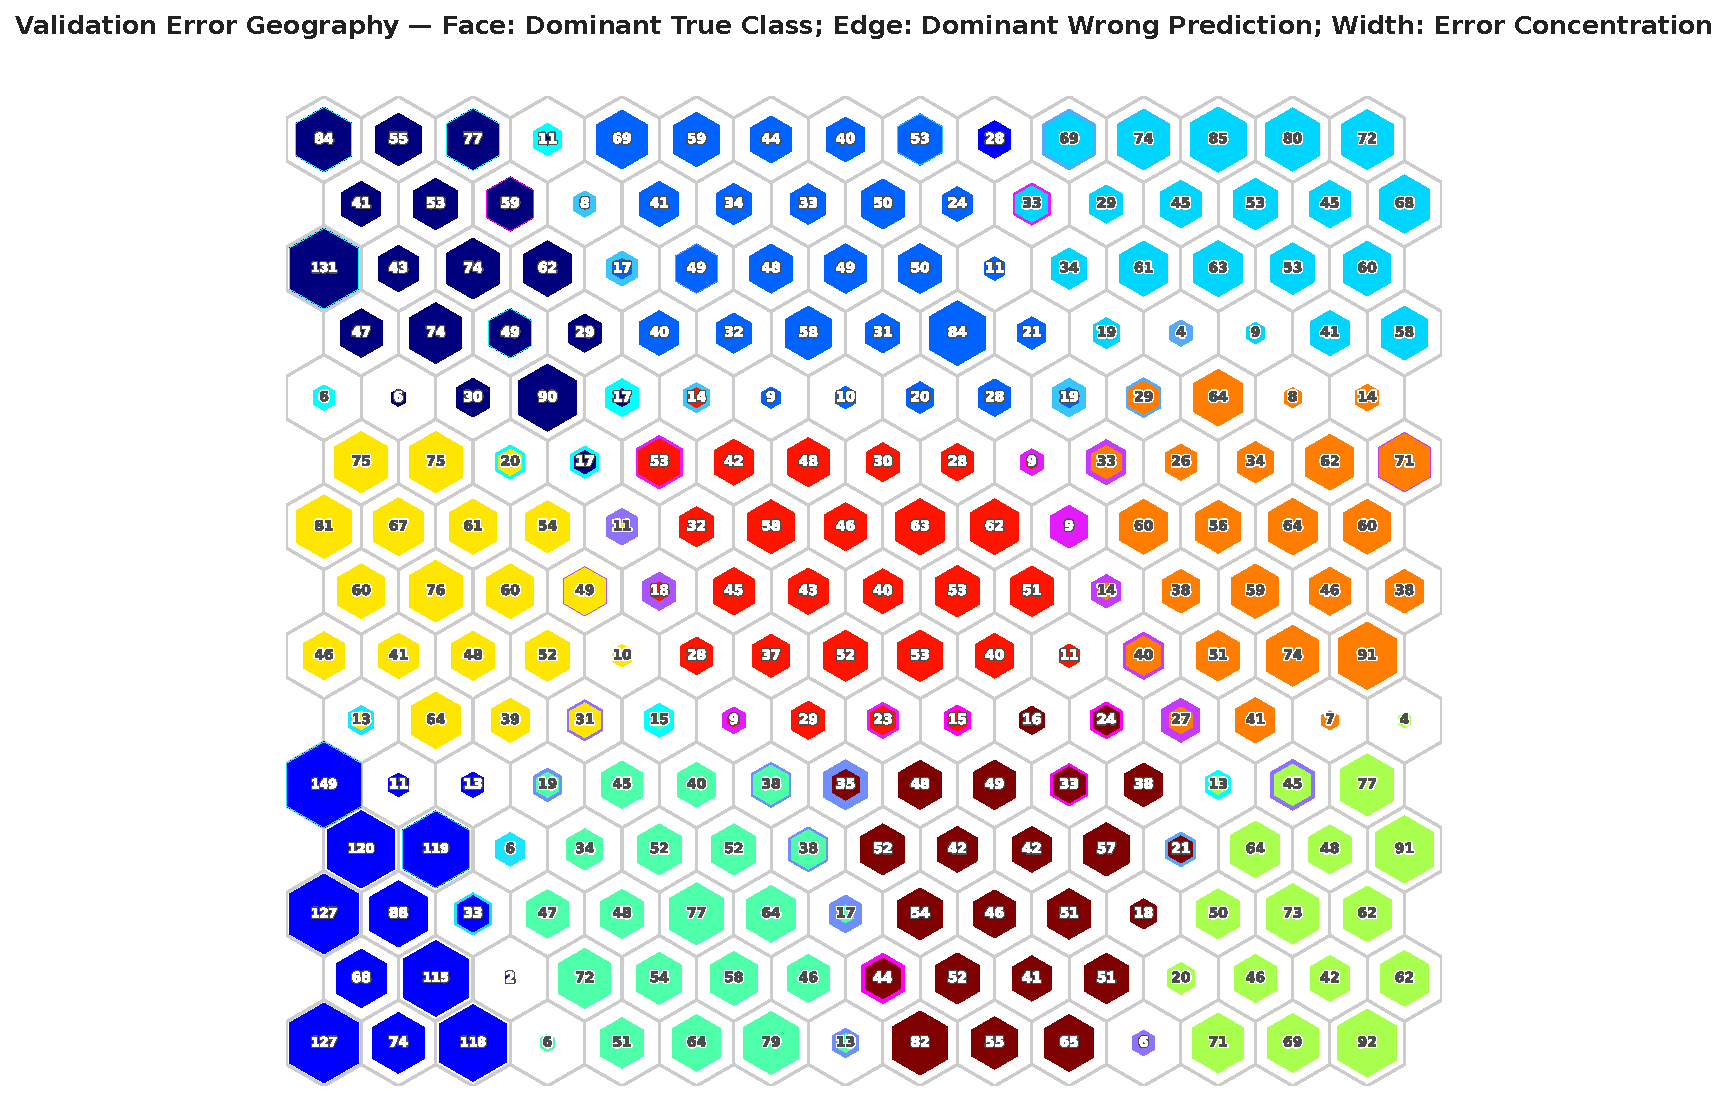
\includegraphics[width=\linewidth,keepaspectratio]{mnist_p2_validation_complex_error_map.pdf}\\{\small (a) MNIST}
\end{minipage}\hfill
\begin{minipage}[c]{0.49\textwidth}\centering
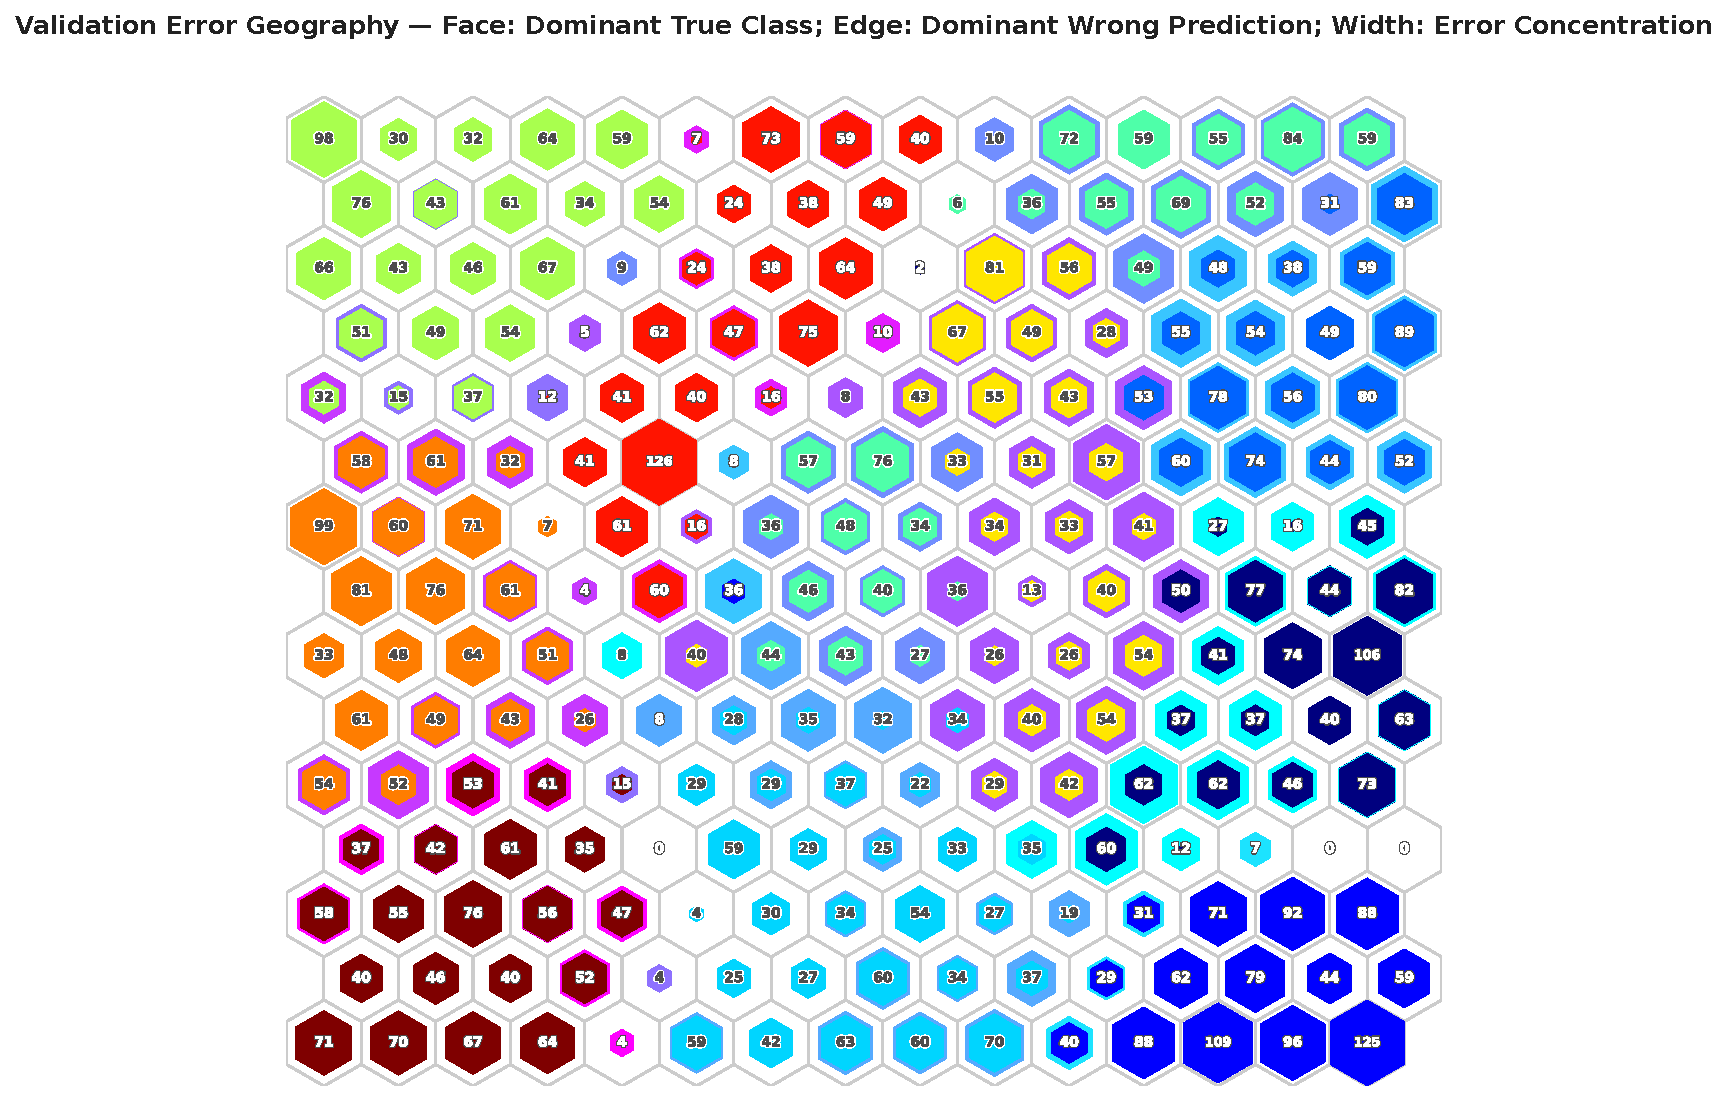
\includegraphics[width=\linewidth,keepaspectratio]{fashion_mnist_p2_validation_complex_error_map.pdf}\\{\small (b) Fashion-MNIST}
\end{minipage}
\caption{Validation error maps of the 15$\times$15 SOMs. Fill: most common true class of the cell; edge colour: most common wrong answer; size: number of mistakes.}
\label{fig:errormaps}
\end{figure}

\begin{figure}[H]
\centering
\begin{minipage}[c]{0.45\textwidth}\centering
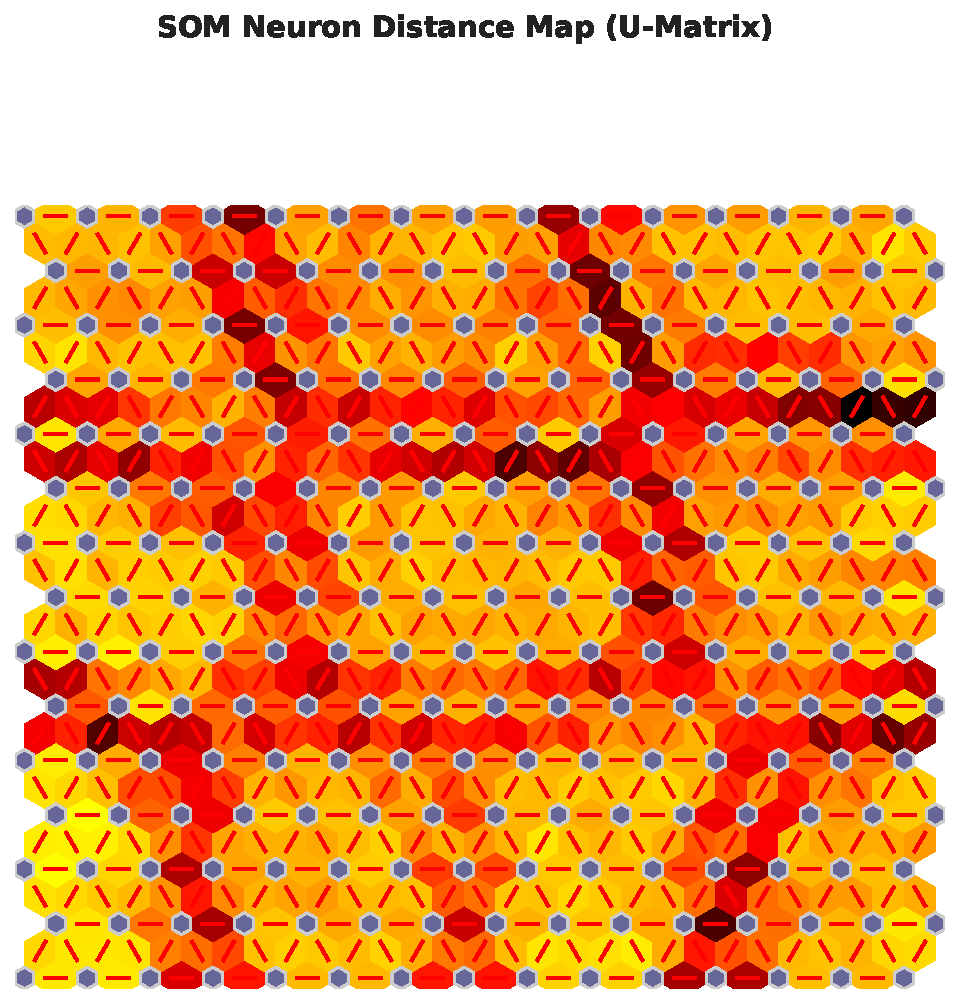
\includegraphics[width=\linewidth,keepaspectratio]{mnist_p2_u_matrix.pdf}\\{\small (a) MNIST}
\end{minipage}\hfill
\begin{minipage}[c]{0.45\textwidth}\centering
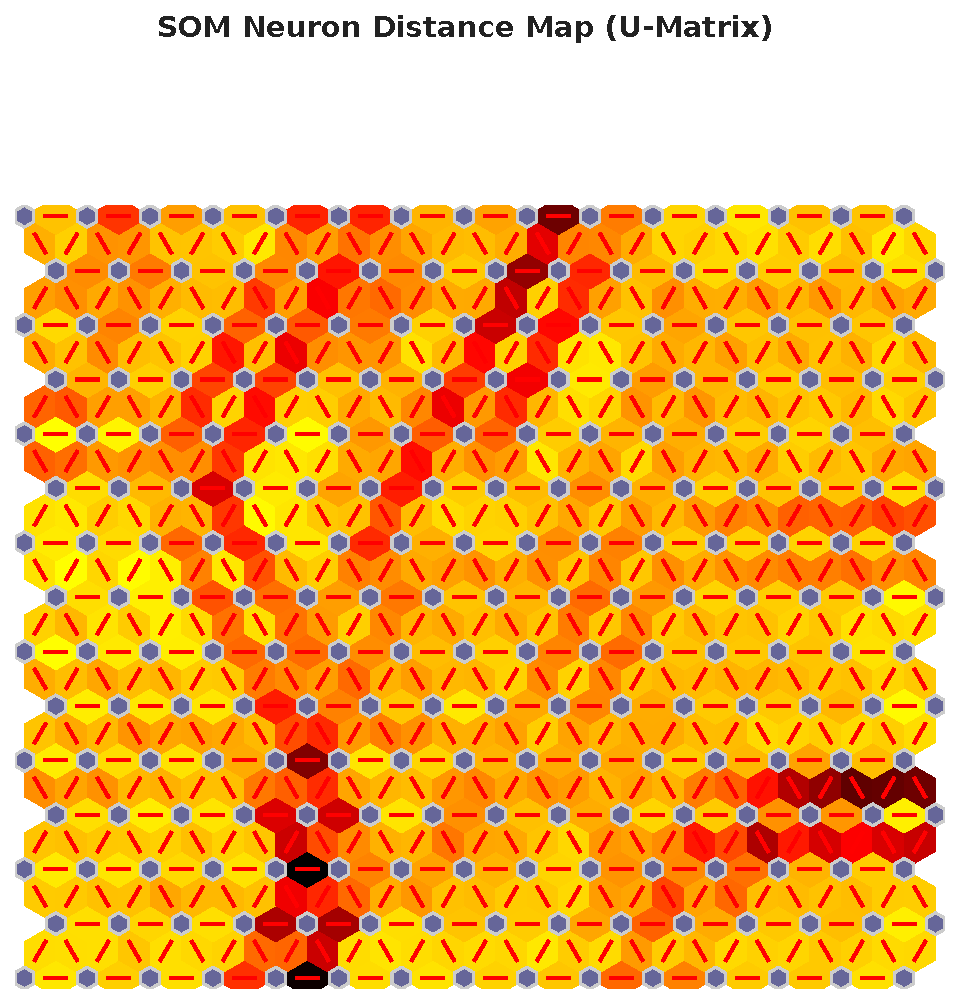
\includegraphics[width=\linewidth,keepaspectratio]{fashion_mnist_p2_u_matrix.pdf}\\{\small (b) Fashion-MNIST}
\end{minipage}
\caption{U-matrices: distance between neighbouring cells; high values mark borders between groups of cells. On Fashion-MNIST the strongest borders surround the footwear, while the clothing part has weak borders.}
\label{fig:umatrix}
\end{figure}

Figure~\ref{fig:overlay} shows where the SVHN images are mapped. On both datasets they collapse onto a few cells within a single class region. This view, which a single scalar score does not convey, indicates which known class the novel images most resemble in the network's feature space.

\begin{figure}[H]
\centering
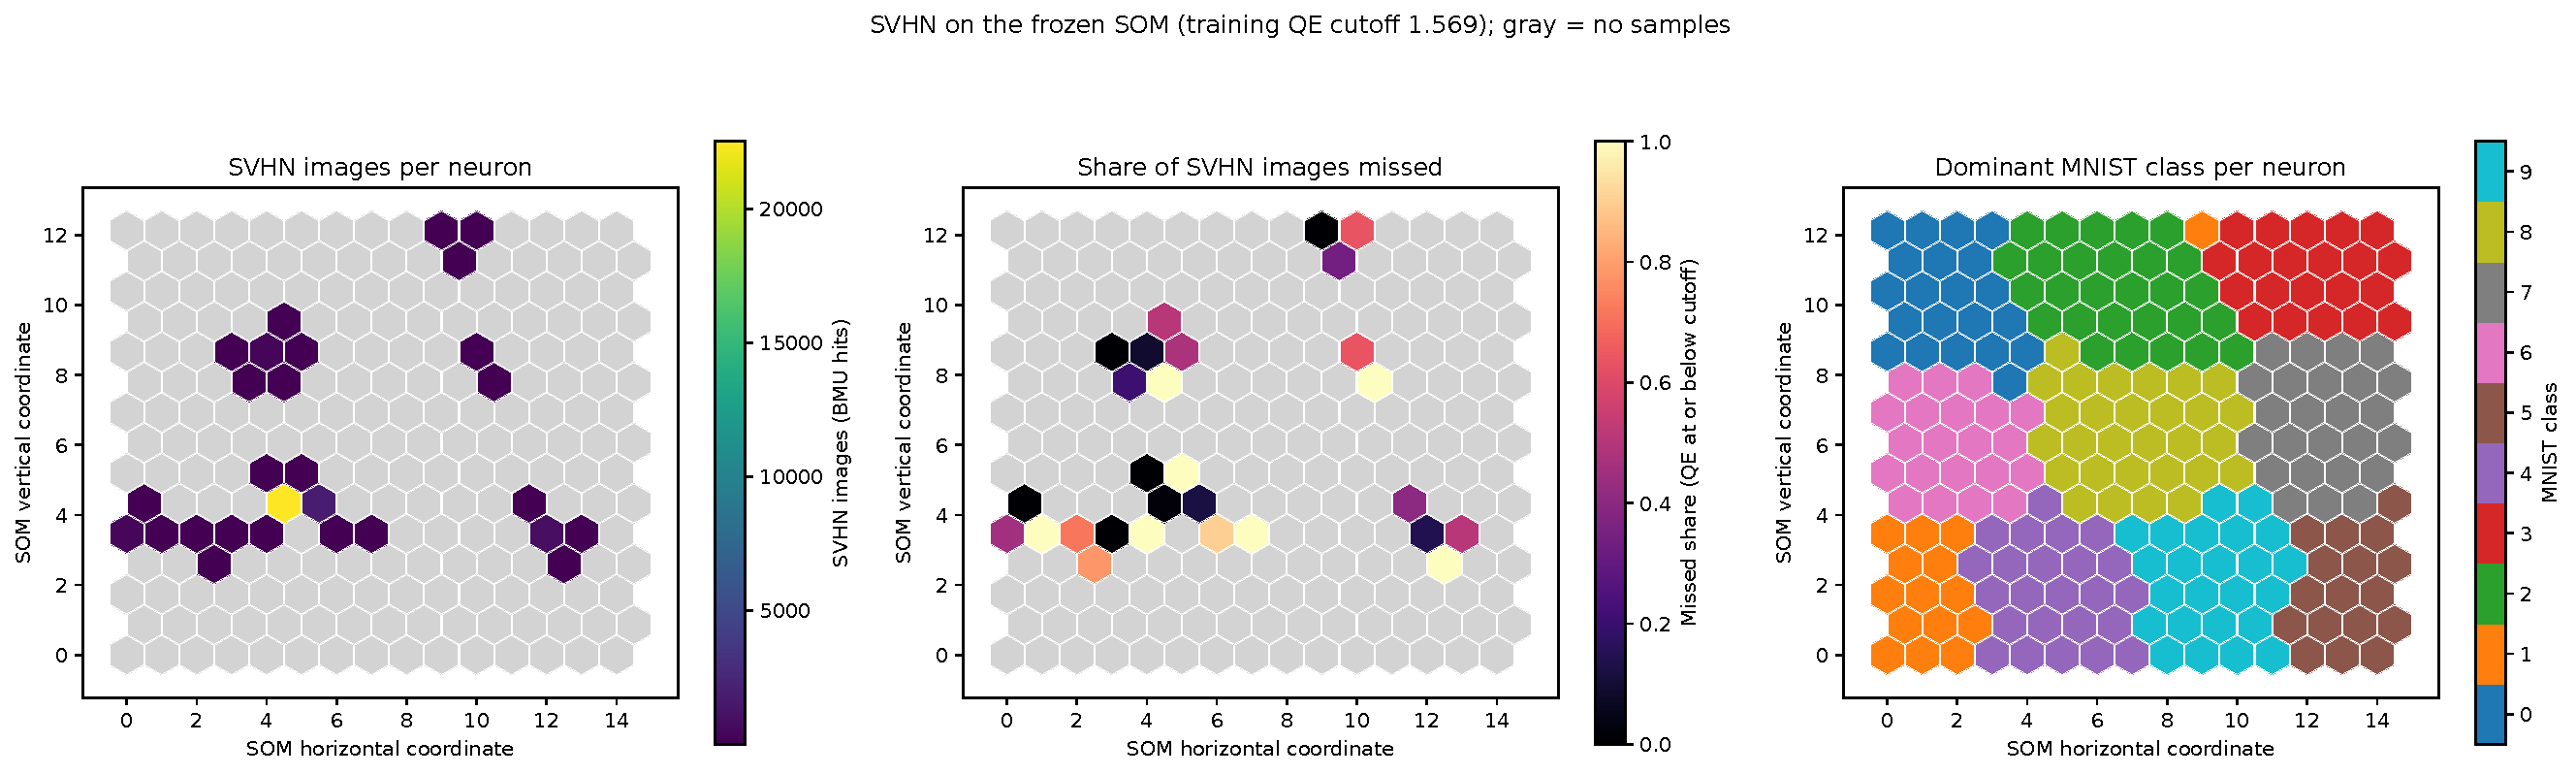
\includegraphics[width=0.92\textwidth,keepaspectratio]{mnist_p3_svhn_som_overlay.pdf}\\{\small (a) MNIST: 28 cells; one cell of digit 4 receives 86.5\%}\\[4pt]
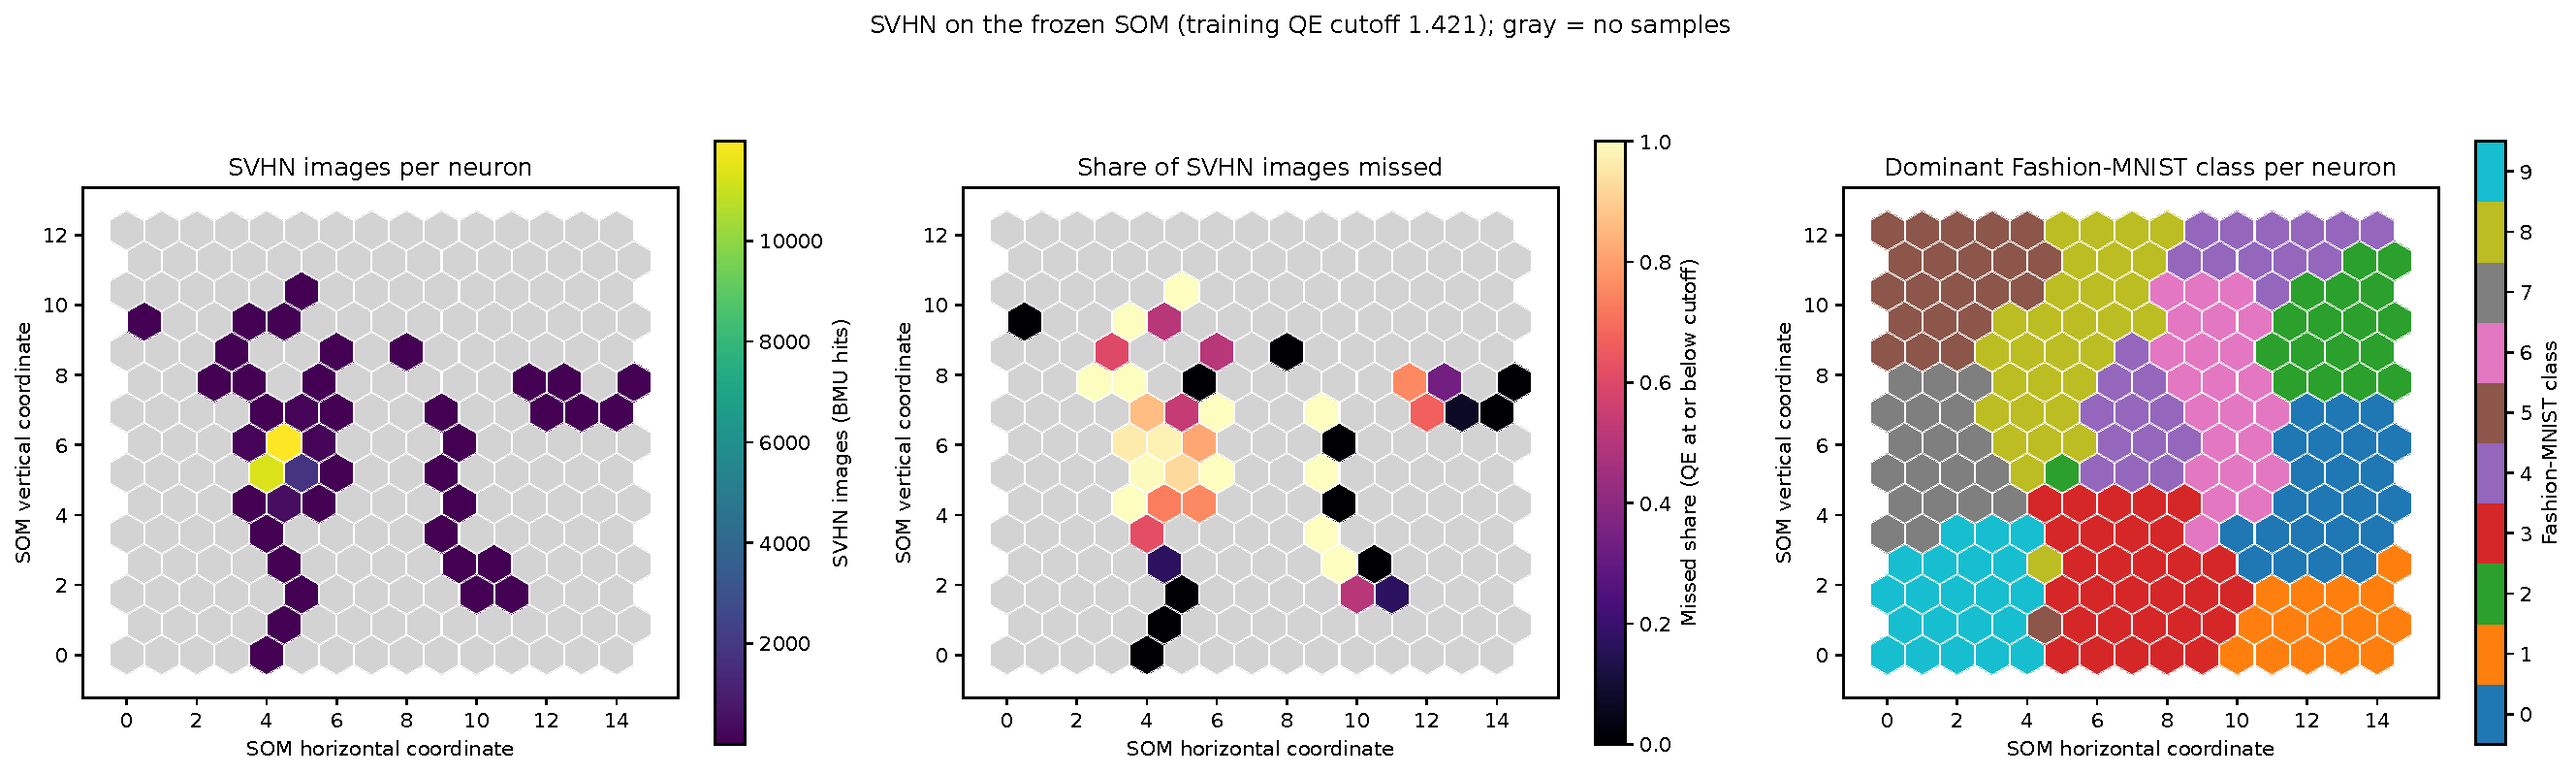
\includegraphics[width=0.92\textwidth,keepaspectratio]{fashion_mnist_p3_svhn_som_overlay.pdf}\\{\small (b) Fashion-MNIST: 42 cells, mostly the Bag region}
\caption{SVHN test images on the 15$\times$15 SOMs: images per cell, share missed at the fixed threshold, and the most common class of each cell. Descriptive only.}
\label{fig:overlay}
\end{figure}

Figure~\ref{fig:reanalysis} reports the measures of the new SOMs for each seed. On MNIST, the hotspots of the SOM-guided arm contain fewer errors than after normal training in every seed; on Fashion-MNIST they do not, and the new maps are less pure.

\begin{figure}[H]
\centering
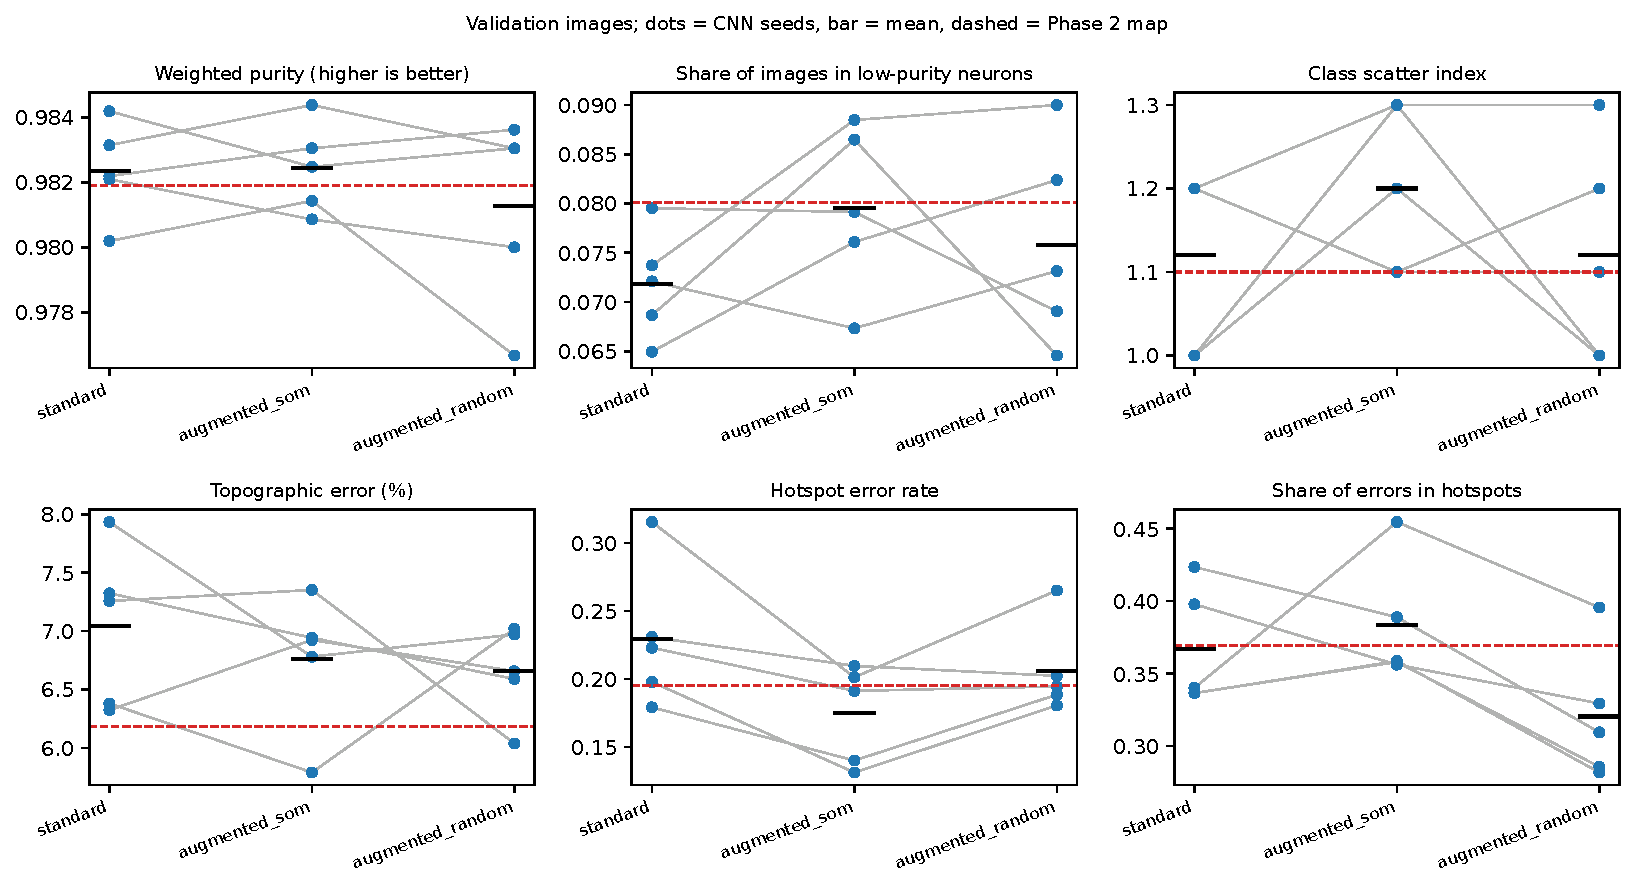
\includegraphics[width=0.92\textwidth]{mnist_p4_map_measures_by_arm.pdf}\\{\small (a) MNIST}\\[4pt]
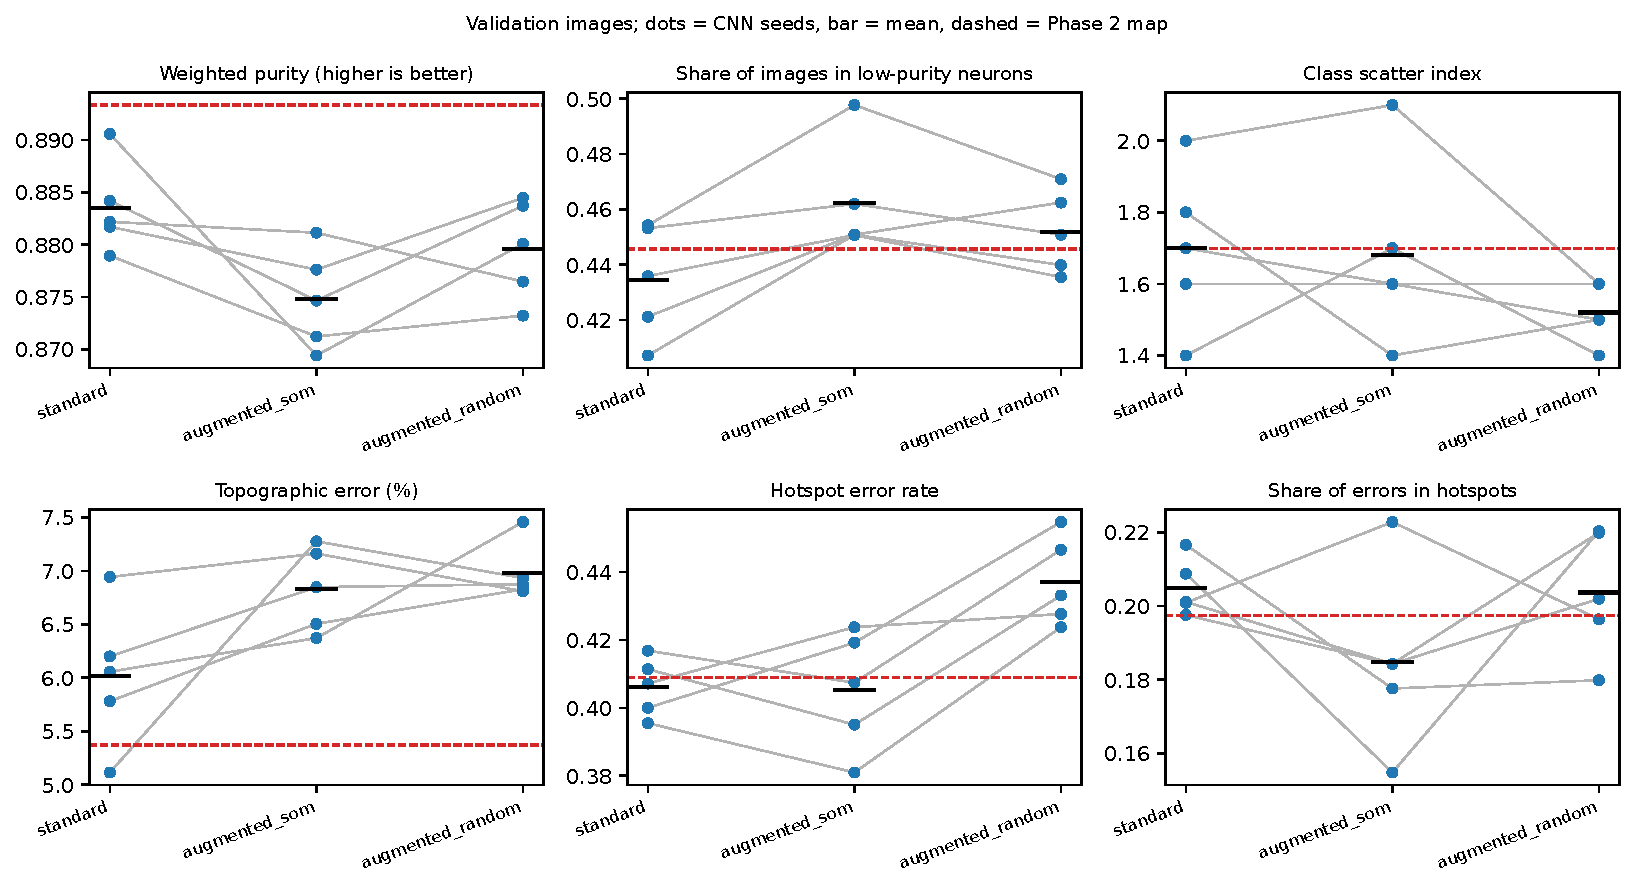
\includegraphics[width=0.92\textwidth]{fashion_mnist_p4_map_measures_by_arm.pdf}\\{\small (b) Fashion-MNIST}
\caption{Measures of the new SOMs after retraining, on validation images. Each dot is one CNN seed, the black bar is the mean over seeds, and the dashed line is the original (Phase 2) map.}
\label{fig:reanalysis}
\end{figure}

Figure~\ref{fig:cf} compares CF1 and CF2. On MNIST, a few confusions become less frequent. On Fashion-MNIST, the main change is an exchange of errors between Shirt and T-shirt/top, with almost no net improvement (Table~\ref{tab:endtoend}).

\begin{figure}[H]
\centering
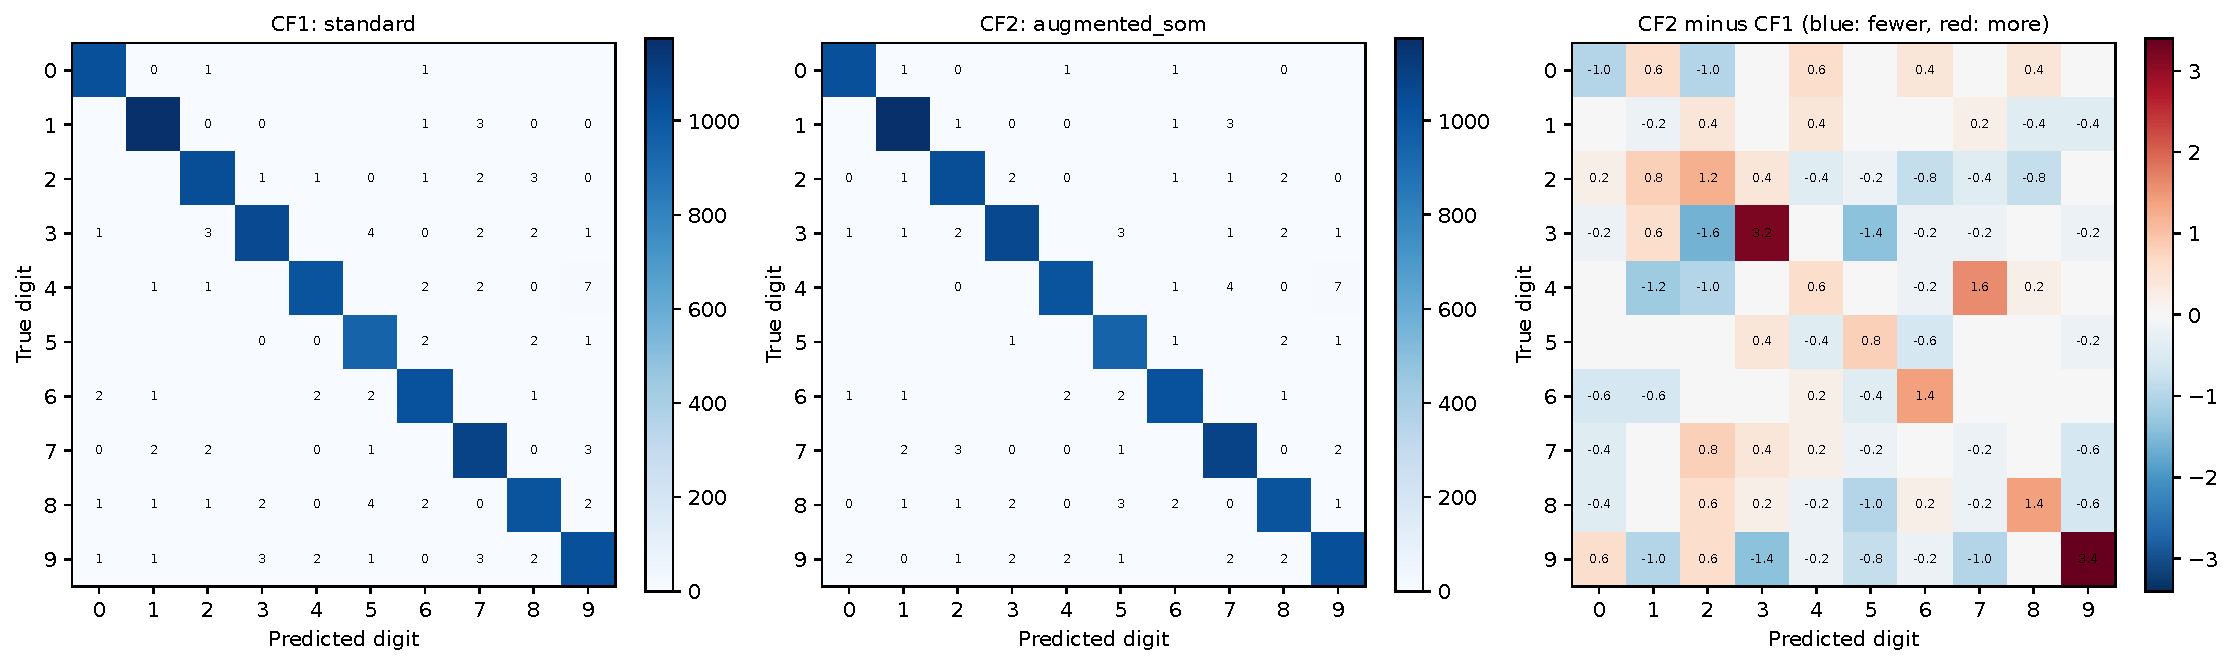
\includegraphics[width=0.92\textwidth]{mnist_p4_confusion_standard_vs_augmented_som.pdf}\\{\small (a) MNIST}\\[4pt]
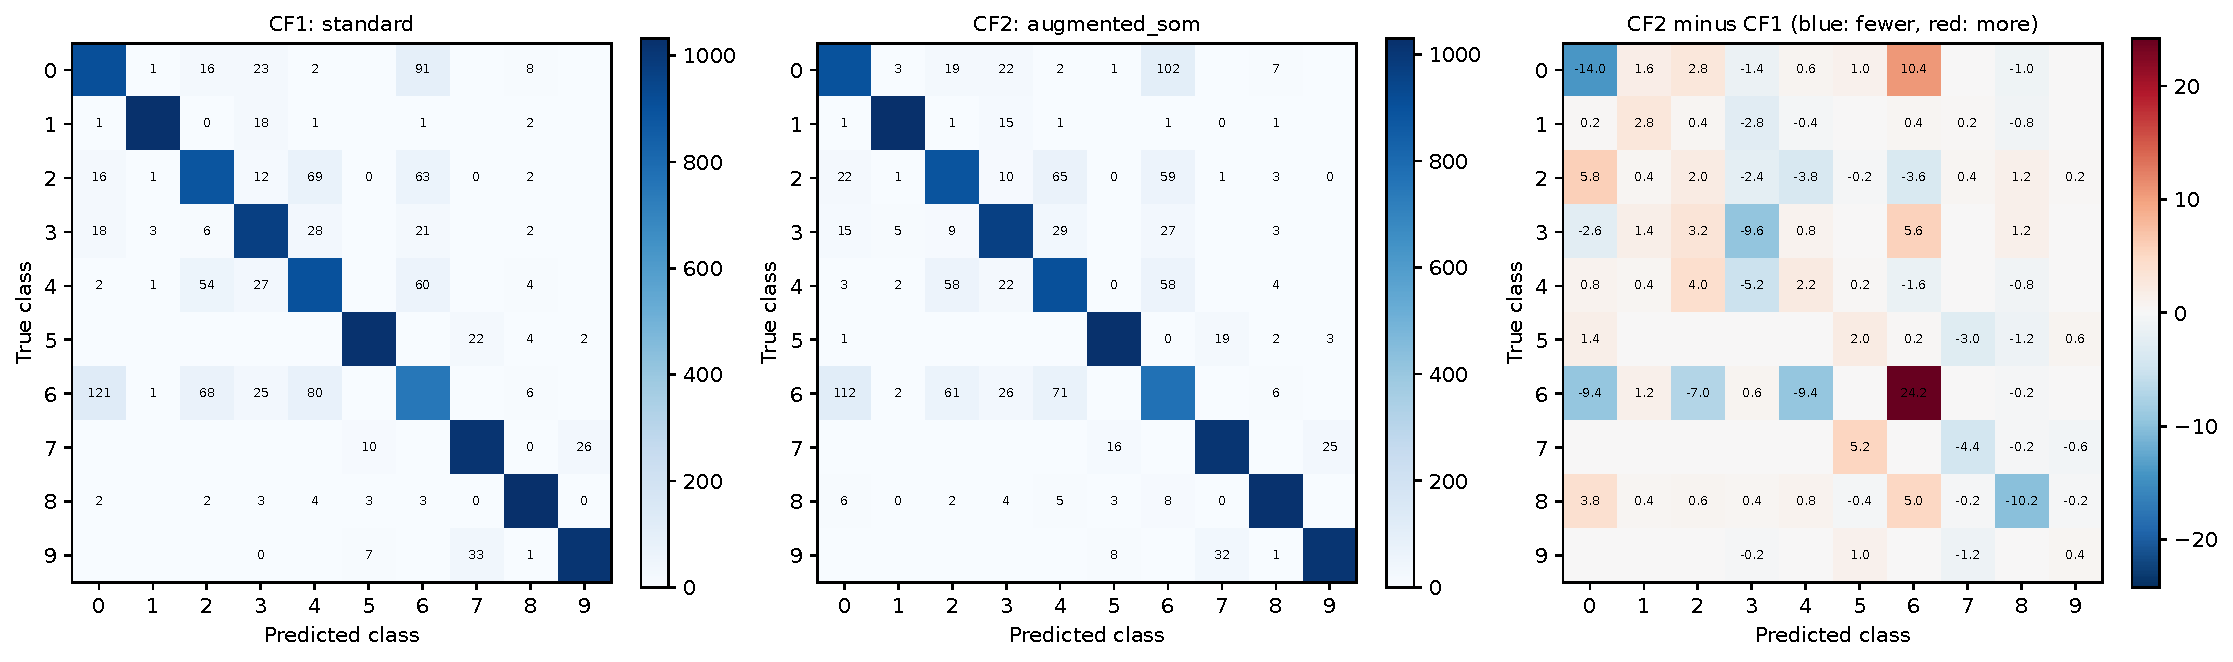
\includegraphics[width=0.92\textwidth]{fashion_mnist_p4_confusion_standard_vs_augmented_som.pdf}\\{\small (b) Fashion-MNIST}
\caption{CF1 (normal training) and CF2 (SOM-guided augmentation): mean test confusion matrices over 5 seeds and their difference (blue: fewer cases, red: more).}
\label{fig:cf}
\end{figure}

% ------------------------------------------------------------------------------------------------------------------------
\section{Discussion}\label{sec:discussion}

\textbf{Main contribution.} On MNIST, the SOM was as effective as the network's own confidence for guiding retraining and, unlike the confidence score, it also showed where the errors cluster and why: in a few cells where two classes overlap. On Fashion-MNIST the same design no longer improved retraining, but the map still identified the group of classes that the network cannot separate.

\textbf{The SOM's contribution is the map, not the score.} As a scoring method, the SOM does not outperform the strongest simple baselines on either dataset, although its quantization error is better than the Mahalanobis distance on both datasets for SVHN. For error detection, the SOM cell error rate (AUROC 0.685 on MNIST and 0.811 on Fashion-MNIST) is no better than k-means clustering (0.693 and 0.812) and is clearly worse than the network's maximum softmax probability (0.981 and 0.906). For far novelty detection, the SOM's quantization error (0.981 and 0.789) is below both the energy score (0.9998 and 0.982) and the maximum softmax probability (0.9985 and 0.884). The only setting in which a SOM score outperforms the network's confidence is the detection of unseen clothing classes on Fashion-MNIST (Table~\ref{tab:near}), and even there the nearest-neighbour distance is better. We therefore do not present the SOM as a better detector. Its contribution is the map itself: a single, topology-preserving view of the feature space that shows where errors concentrate, which classes overlap, and where novel inputs are placed, information that a single scalar score does not convey. Figure~\ref{fig:errormaps} shows this most directly: the cells with many mistakes lie where two classes meet, which is also where the hard-example pool for retraining is drawn from (hotspot and low-purity cells, together with images far from their best cell). Figure~\ref{fig:overlay} shows the same for novel inputs, which collapse onto a few cells of a single known class region.

\textbf{What the SOM reveals beyond standard metrics.}
\begin{itemize}
  \item \textbf{The location and nature of errors.} Accuracy and the confusion matrix indicate how many errors occur and between which classes. The map additionally shows that the errors lie in regions where classes overlap and how large these regions are: a few small cells with atypical handwriting on MNIST, and one broad region of upper-body garments on Fashion-MNIST.
  \item \textbf{How novel inputs are represented.} SVHN images collapse onto one cell of the digit 4 on MNIST and onto the Bag region on Fashion-MNIST, where the map treats them as typical bags. Together with the embedding-length effect, this helps explain why a fixed QE threshold works on one dataset and fails on the other.
  \item \textbf{Unseen classes of a similar kind.} On Fashion-MNIST the map detects unseen clothing classes better than the network's confidence, which is the setting closest to practical use.
\end{itemize}

\textbf{Where simpler methods perform better.}
\begin{itemize}
  \item For error detection, the network's confidence is clearly superior and k-means is equally good.
  \item For far novelty, the energy score and the maximum softmax probability are superior on both datasets, and the SVHN results are largely explained by embedding length.
  \item For near novelty, the nearest-neighbour distance on the same embeddings outperforms the map on both datasets.
  \item For selecting retraining images, the least-confident images are as effective as SOM-selected ones.
\end{itemize}

\textbf{Challenges and how they were addressed.}
\begin{itemize}
  \item \emph{Few errors on MNIST:} the study was replicated on Fashion-MNIST, where the grid comparison was decisive and the intervals are narrower.
  \item \emph{Patterns that might not be specific to the SOM:} each finding is accompanied by a permutation control and by simple baselines on the same embeddings.
  \item \emph{Augmentations that altered the class:} the ranges were checked before training and reduced according to rules recorded before each new check.
  \item \emph{Inverted novelty detectors:} the embedding-length diagnostics explained the behaviour, and no score was inverted after the labels were seen.
\end{itemize}

\textbf{Limitations.}
\begin{itemize}
  \item LeNet-5 is the only CNN studied. The findings describe how the SOM behaves on the features of this small network, and we did not test whether they hold for deeper architectures such as ResNet.
  \item The headline Phase 2 and Phase 3 results use one network and one SOM seed; the SOM seed alone changes the Fashion-MNIST SVHN AUROC by about 0.1.
  \item MNIST yields only 92 validation errors, so differences smaller than about 0.1 AUROC cannot be detected.
  \item SVHN is the only out-of-distribution dataset, and it differs mainly in embedding length, also after retraining. The near-novelty experiment uses held-out classes of the same dataset; the splits share images and classes, so their $t$-intervals may be too narrow, and the random draw left the classes unbalanced (both datasets use the same class indices; class 5, the digit 5 or Sandal, is unknown in all five splits and class 9 in none).
  \item The baseline comparison covers only the $15\times15$ map, and on MNIST it uses three k-means initialisations per seed.
  \item The first augmentation settings failed the pre-training check on both datasets (MNIST: 99.12\% to 95.83\% with 2-pixel translations; Fashion-MNIST: 91.66\% to 83.60\%, then 88.76\%) and were reduced according to recorded rules.
  \item In Phase 4 the hotspots are defined by the SOM, which favours the SOM-guided arms on hotspot error; the pools come from a single SOM; and five seeds can only resolve relatively large differences.
  \item All Fashion-MNIST settings were copied from MNIST by design, so the pool rule and the curriculum schedule were not adapted to a dataset with many more errors.
  \item The validation set was also used to select the network checkpoint.
\end{itemize}

\textbf{Recommendations.} The hard-example rule and the curriculum schedule should be selected for each dataset on validation data, under a new protocol, so that the pool remains selective. When far-novelty detection is the goal, the earlier fc1 layer or the nearest-neighbour distance should be preferred. A near-novelty test should also be carried out on the retrained networks.

% ------------------------------------------------------------------------------------------------------------------------
\section{Conclusion}\label{sec:conclusion}

We used a SOM trained on the embeddings of a fixed CNN as a post-training analysis tool on MNIST and Fashion-MNIST, and tested every claim against chance and simple baselines. Table~\ref{tab:summary} summarises the results for each objective of the proposal.

\begin{table}[H]
\centering
\caption{Project Objectives and Findings}
\label{tab:summary}
\renewcommand{\arraystretch}{1.12}
\footnotesize
\begin{tabular}{|L{0.30\textwidth}|L{0.62\textwidth}|}
\hline
\textbf{Objective} & \textbf{Result} \\ \hline
Baseline model and benchmarks & LeNet-5: 99.18\% (MNIST) and 90.90\% (Fashion-MNIST) test accuracy, with per-class F1 and confusion matrices. \\ \hline
Feature extraction and SOM & fc2 embeddings of every image; 15$\times$15 NNSOM maps, chosen and checked by a grid comparison, an Optuna check and a feature-layer ablation. \\ \hline
Cluster structure and error patterns & Classes form regions far beyond chance; mistakes gather where classes overlap (3.9 to 11 times their share). The SOM finds mistakes no better than k-means, and worse than the network's confidence. \\ \hline
Novelty detection & QE detects SVHN (0.981 and 0.789) but energy is better; the SOM beats max-softmax on unseen clothing classes (+0.046). \\ \hline
Guided retraining & SOM-guided augmentation reduced hotspot mistakes on MNIST (11.4\% to 7.8\%) but not clearly on Fashion-MNIST; least-confident images work as well; curriculum learning hurt on both. \\ \hline
Reusable pipeline & The same code and protocol ran on both datasets with only the forced changes recorded. \\ \hline
\end{tabular}

\end{table}

The contribution of the SOM is the map, not its scores. It is most valuable as an \emph{explanatory} tool: it shows where, and between which classes, a network fails, and where unfamiliar inputs are mapped. It does not detect errors or far out-of-distribution inputs better than the network's own scores, and it does not select retraining images better than the network's confidence. Future work should adapt the hard-example rule and the curriculum to each dataset under a new protocol, repeat the near-novelty experiment after retraining, and test the findings with a deeper network.

\section*{Acknowledgment}

The authors thank Dr.\ Amir Jafari for supervising this project. In preparing this report, the authors used Claude (Anthropic), a large language model, to draw the diagrams in Figs.~\ref{fig:pipeline}--\ref{fig:endtoend} in draw.io (17 November 2026; relabelled for both datasets on 22 November 2026) and to compile Tables~\ref{tab:baseline}--\ref{tab:summary} from the project's experimental results (22 November 2026). All values were checked against the experiment outputs, and the authors take full responsibility for the content of this report.

\bibliographystyle{IEEEtran}
\bibliography{references}

\end{document}
